\makepart{Your turn: Hands-on Deep Learning}

\section{Build and use an autoencoder}

\subsection{Formal introduction of an autoencoder}


\begin{frame}


    \begin{block}{Definition}
        An autoencoder is a type of artificial neural network used to learn efficient codings of unlabeled data. It consists of two main components:
        \begin{itemize}
            \item An \alert{encoder} function: $encoder(x): \mathbb{R}^d \rightarrow \mathbb{R}^m$ \\
                  Maps an input $x$ from the input space $\mathbb{R}^d$ to a hidden representation space $\mathbb{R}^m$.
            \item A \alert{decoder} function: $decoder(z): \mathbb{R}^m \rightarrow \mathbb{R}^d$ \\
                  Maps the hidden representation $z$ back to the original input space $\mathbb{R}^d$.
        \end{itemize}
    \end{block}

    \begin{block}{Goal}
        The primary goal of an autoencoder is to learn a representation (encoding) for a set of data, typically for the purpose of dimensionality reduction or feature learning. Through training, the autoencoder learns to compress the data from $\mathbb{R}^d$ to $\mathbb{R}^m$ (where $m < d$) and then reconstruct the data back to $\mathbb{R}^d$ as accurately as possible. This process forces the autoencoder to capture the most important features of the data in the hidden representation $z$.
    \end{block}
\end{frame}

\begin{frame}
    \begin{figure}
        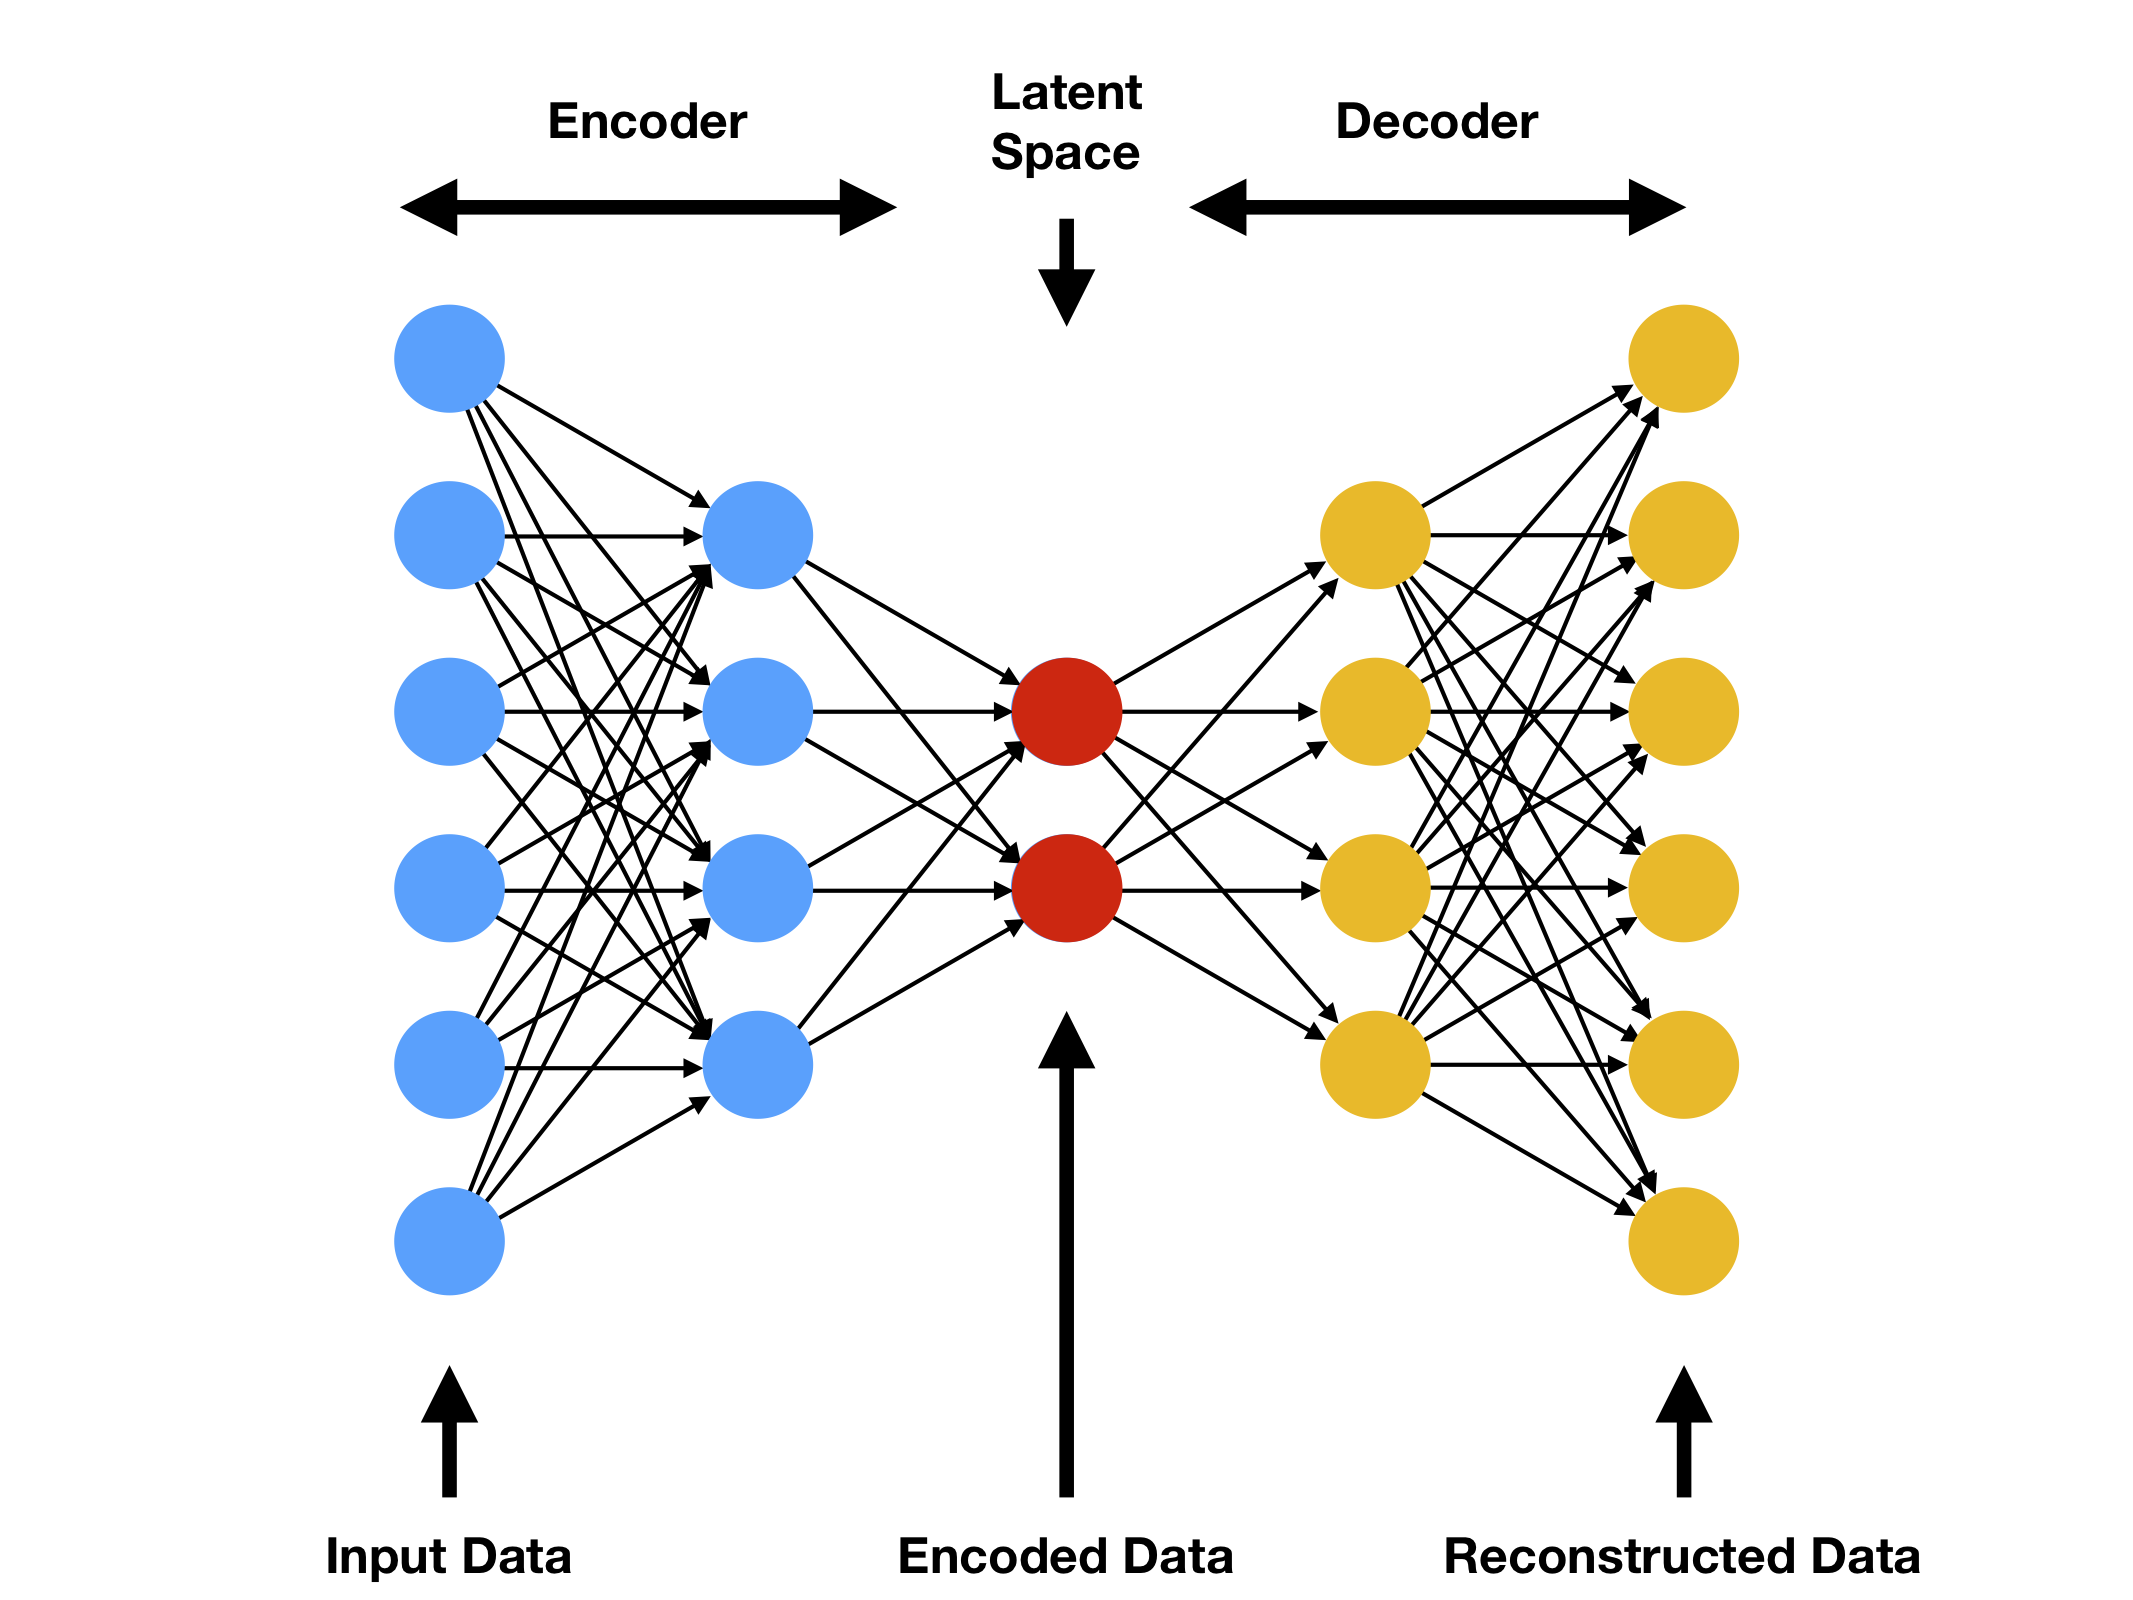
\includegraphics[width=0.7\textwidth]{figures/ae.png}
    \end{figure}
\end{frame}


\begin{frame}{}{Autoencoders and Unsupervised Learning}

    \begin{block}{Unsupervised Learning}
        Autoencoders are a classic example of \alert{unsupervised learning}. In unsupervised learning, the goal is to learn patterns from unlabelled data. Autoencoders learn to compress and decompress the input data without any explicit labels, aiming to capture the underlying structure of the data.
    \end{block}

    \begin{block}{Objective Function}
        The learning process of an autoencoder is guided by the minimization of a loss function, typically involving a norm that measures the difference between the input and the reconstructed output. Formally, the objective is to minimize:

        \[
            \min_{\theta} \; \E_{x \sim P} \left[l(x, \mathrm{decoder}_\theta(\mathrm{encoder}_\theta(x)))\right]
        \]

        where \(x\) is the input data, \(\theta\) represents the parameters of the encoder and decoder, and $l$ is a loss function.
    \end{block}

\end{frame}

\begin{frame}{}{Autoencoders and Unsupervised Learning}

    \begin{block}{Unsupervised Learning}
        Autoencoders are a classic example of \alert{unsupervised learning}. In unsupervised learning, the goal is to learn patterns from unlabelled data. Autoencoders learn to compress and decompress the input data without any explicit labels, aiming to capture the underlying structure of the data.
    \end{block}

    \begin{block}{Objective Function}
        The learning process of an autoencoder is guided by the minimization of a loss function, typically involving a norm that measures the difference between the input and the reconstructed output. Formally, the objective is to minimize:

        \[
            \min_{\theta} \; \E_{x \sim P} \left[\Vert x -  \hat{x} \Vert_2^2\right]
        \]

        where \(x\) is the input data, \(\theta\) represents the parameters of the encoder and decoder and $\hat{x}=\mathrm{decoder}_\theta(\mathrm{encoder}_\theta(x))$ in the reconstruction.
    \end{block}

\end{frame}



\subsection{Applications of U-Net}


\begin{frame}
    \frametitle{Applications of Autoencoders}
    \begin{itemize}
        \item<1-> \textbf{Reduce the size of the data to transfer:} Autoencoders can compress data into a lower-dimensional space, facilitating faster data transfer by reducing the amount of data that needs to be transmitted.
        \item<2-> \textbf{Denoise image:} By learning to ignore the "noise" in the input data, autoencoders can reconstruct cleaner versions of noisy images, effectively removing the noise.
        \item<3-> \textbf{Anomaly detection:} Autoencoders can learn the normal patterns within data. Deviations from these patterns, when the reconstruction error is high, can indicate anomalies or outliers in the data.
    \end{itemize}
    \only<3>{
        \begin{figure}
            \centering
            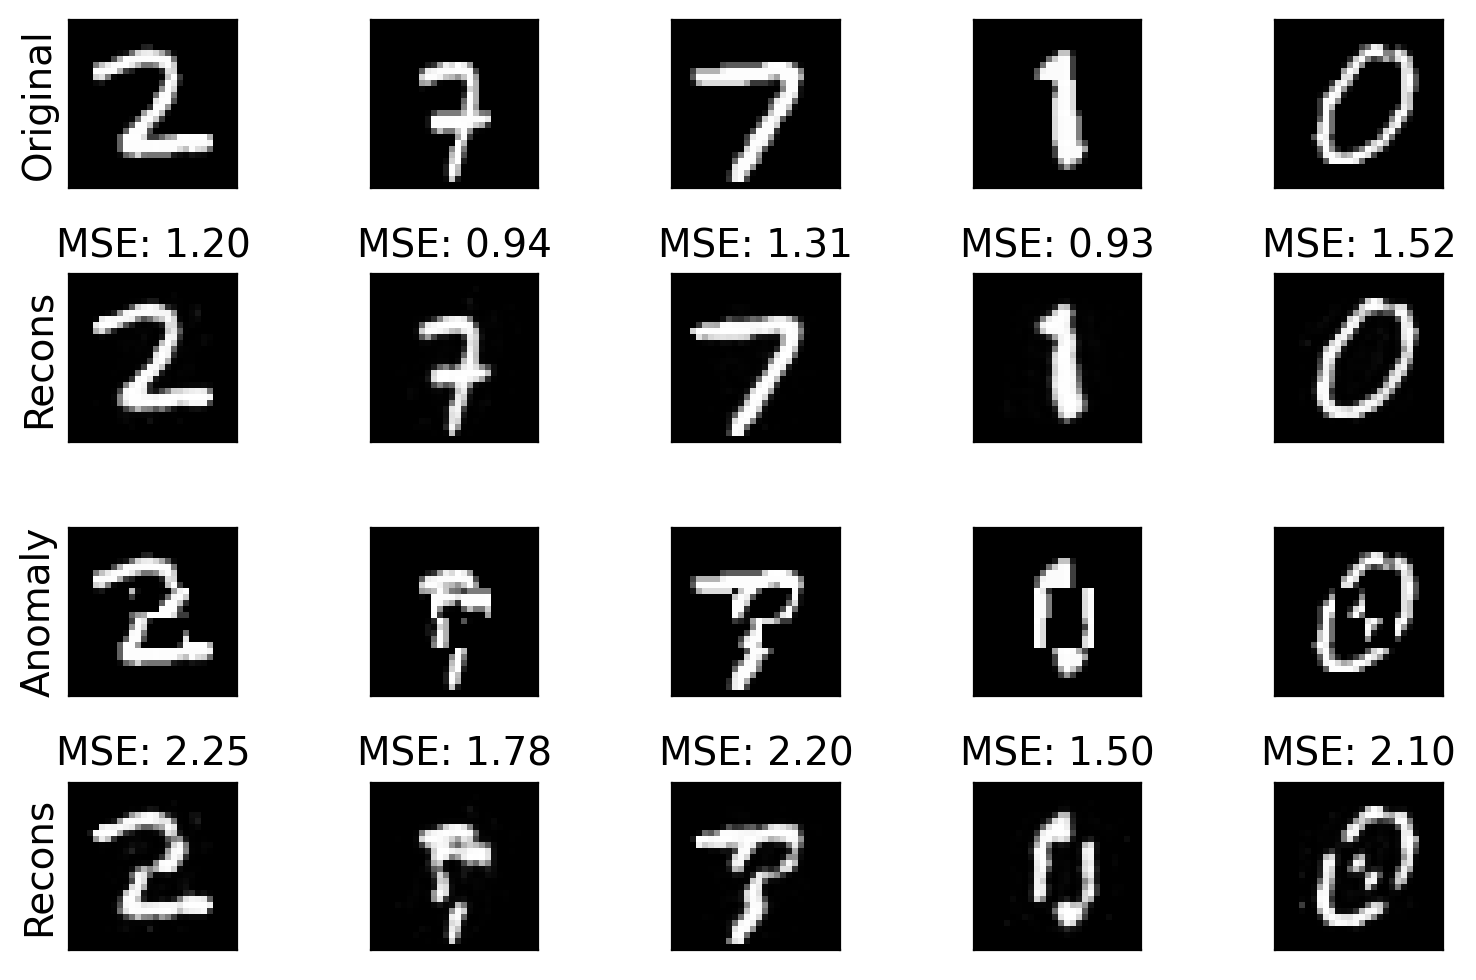
\includegraphics[width=0.5\textwidth]{figures/anomalyimgs.png}
        \end{figure}
    }
    \only<4>{
        \begin{figure}
            \centering
            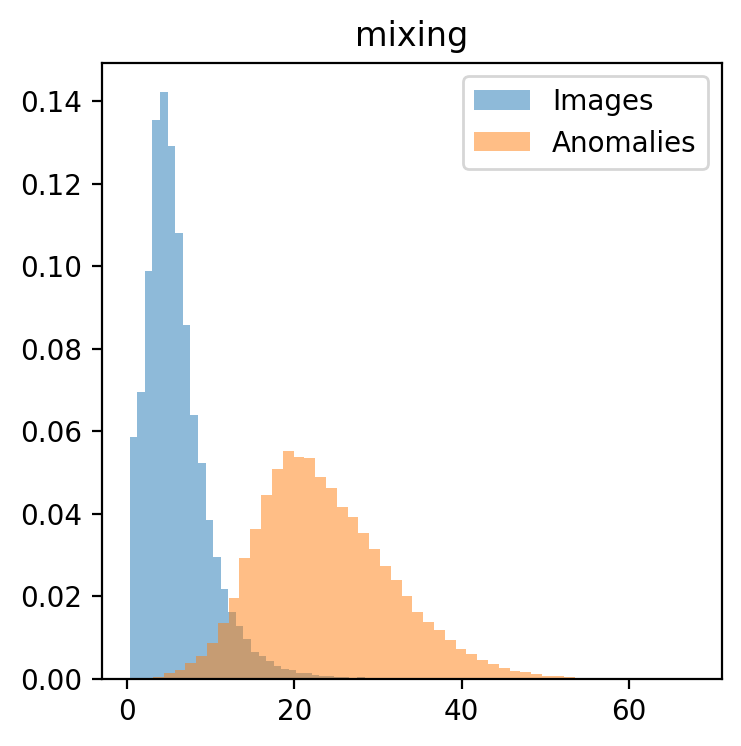
\includegraphics[width=0.35\textwidth]{figures/anoimaly.png}
        \end{figure}
    }
    \only<2>{
        \begin{figure}
            \centering
            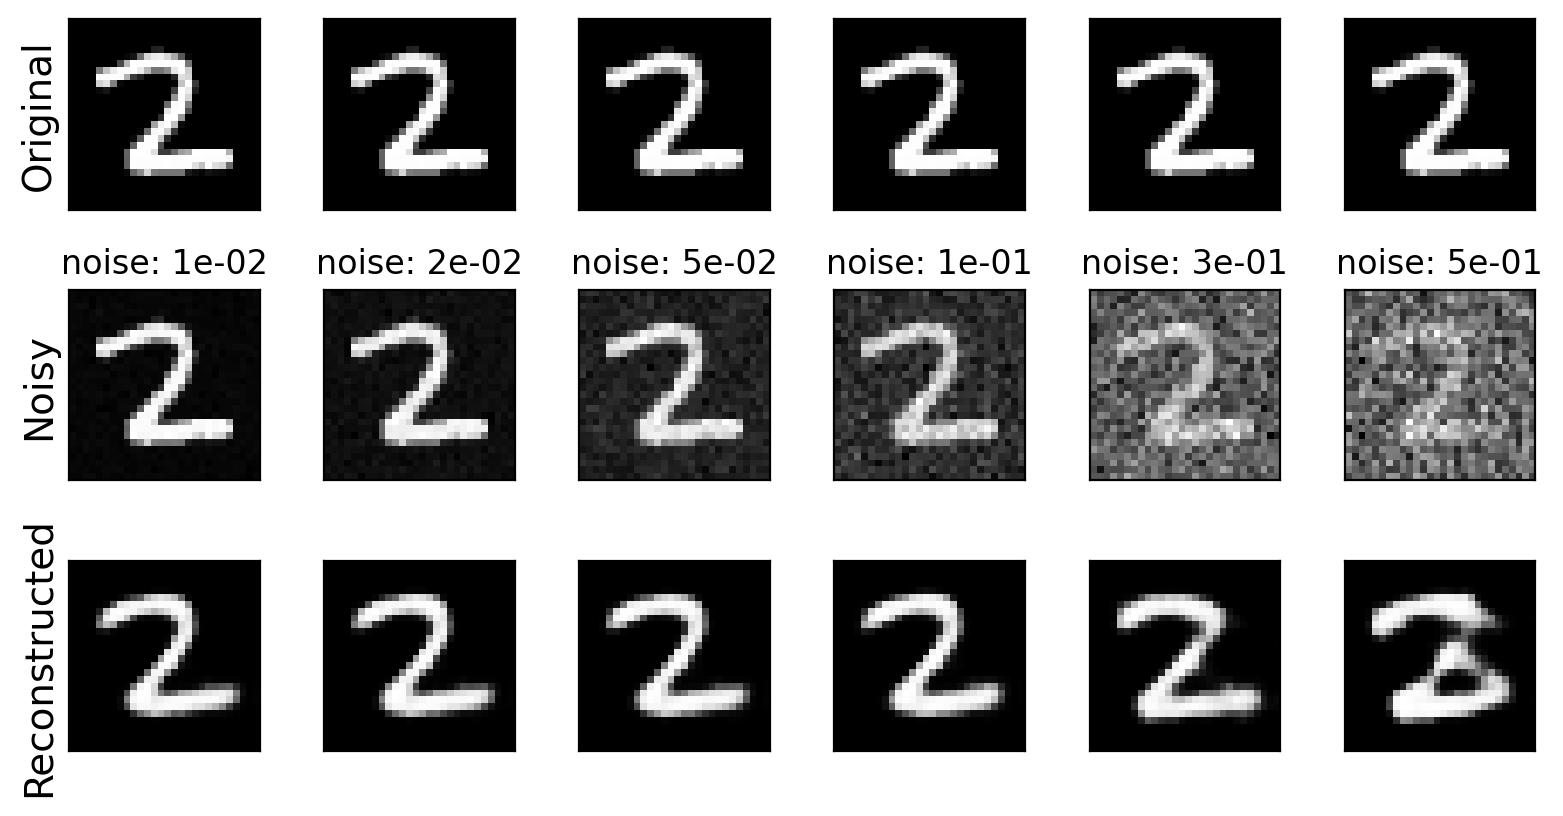
\includegraphics[width=0.6\textwidth]{figures/denoise.png}
        \end{figure}
    }
\end{frame}

\begin{frame}{}{Your turn ! }
    Get the Notebook on the course website and start working on it.
    \begin{itemize}
        \item \url{https://www.alexverine.com}
        \item Teaching
        \item Introduction to Deep Learning
        \item Lien Notebook
    \end{itemize}


\end{frame}



\section{Image Segmentation with U-Net: Correctly evaluate the model}

\subsection{Image Segmentation}

\begin{frame}
    Image segmentation is the process of partitioning an image into multiple segments or regions based on the characteristics of the pixels. It is a fundamental task in computer vision and has applications in various fields, including medical imaging, autonomous driving, and satellite image analysis. There are several methods for image segmentation, including thresholding, clustering, and deep learning-based approaches. In this section, we will focus on a deep learning model called U-Net, which is commonly used for image segmentation tasks.

    \begin{figure}
        \centering
        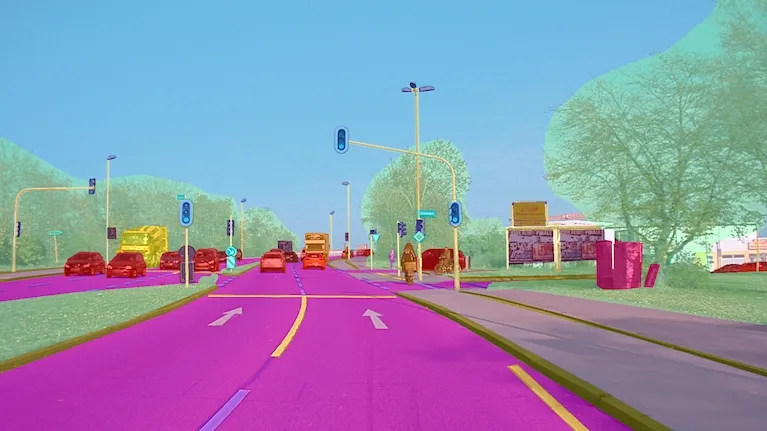
\includegraphics[width = 0.6\textwidth]{figures/imageseg.png}
    \end{figure}
\end{frame}

\begin{frame}{}{Applications of Image Segmentation}
    Image segmentation has a wide range of applications in computer vision and image processing, including:
    \begin{itemize}
        \item Medical Imaging: Segmentation of organs, tumors, and other structures in medical images.
        \item Autonomous Driving: Segmentation of objects such as cars, pedestrians, and road signs in images captured by autonomous vehicles.
        \item Satellite Image Analysis: Segmentation of land cover types, buildings, and other features in satellite images.
        \item Object Detection: Segmentation of objects in images to localize and classify them.
        \item Image Editing: Segmentation of objects for image editing tasks such as background removal and image compositing.
    \end{itemize}
\end{frame}

\begin{frame}{}{Type of Segmentations}
    \begin{minipage}[t]{0.48\textwidth}

        Image segmentation can be broadly classified into two types: semantic segmentation and instance segmentation.
        \begin{itemize}
            \item \textbf{Semantic Segmentation:} Semantic segmentation assigns a class label to each pixel in an image, such as road, car, person, etc. The goal is to partition the image into semantically meaningful regions.
            \item \textbf{Instance Segmentation:} Instance segmentation goes a step further than semantic segmentation by distinguishing between different instances of the same class. It assigns a unique label to each object instance in the image.
        \end{itemize}
    \end{minipage}
    \hfill
    \begin{minipage}[t]{0.48\textwidth}
        \begin{figure}
            \centering
            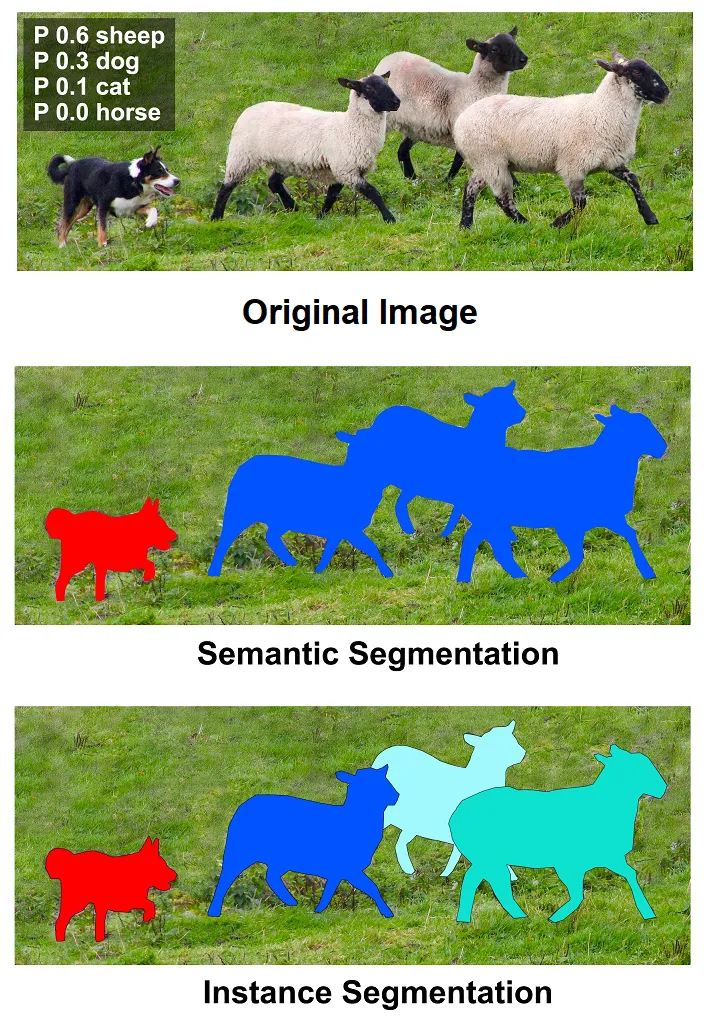
\includegraphics[width = 0.6\textwidth]{figures/typeseg.png}
        \end{figure}
    \end{minipage}
\end{frame}


\subsection{Image Segmentation with U-Net}
\begin{frame}
    U-Net is a convolutional neural network architecture designed for image segmentation tasks. It consists of an encoder-decoder structure with skip connections that allow the model to capture both local and global features in the input image.
    \vfill
    \begin{figure}
        \centering
        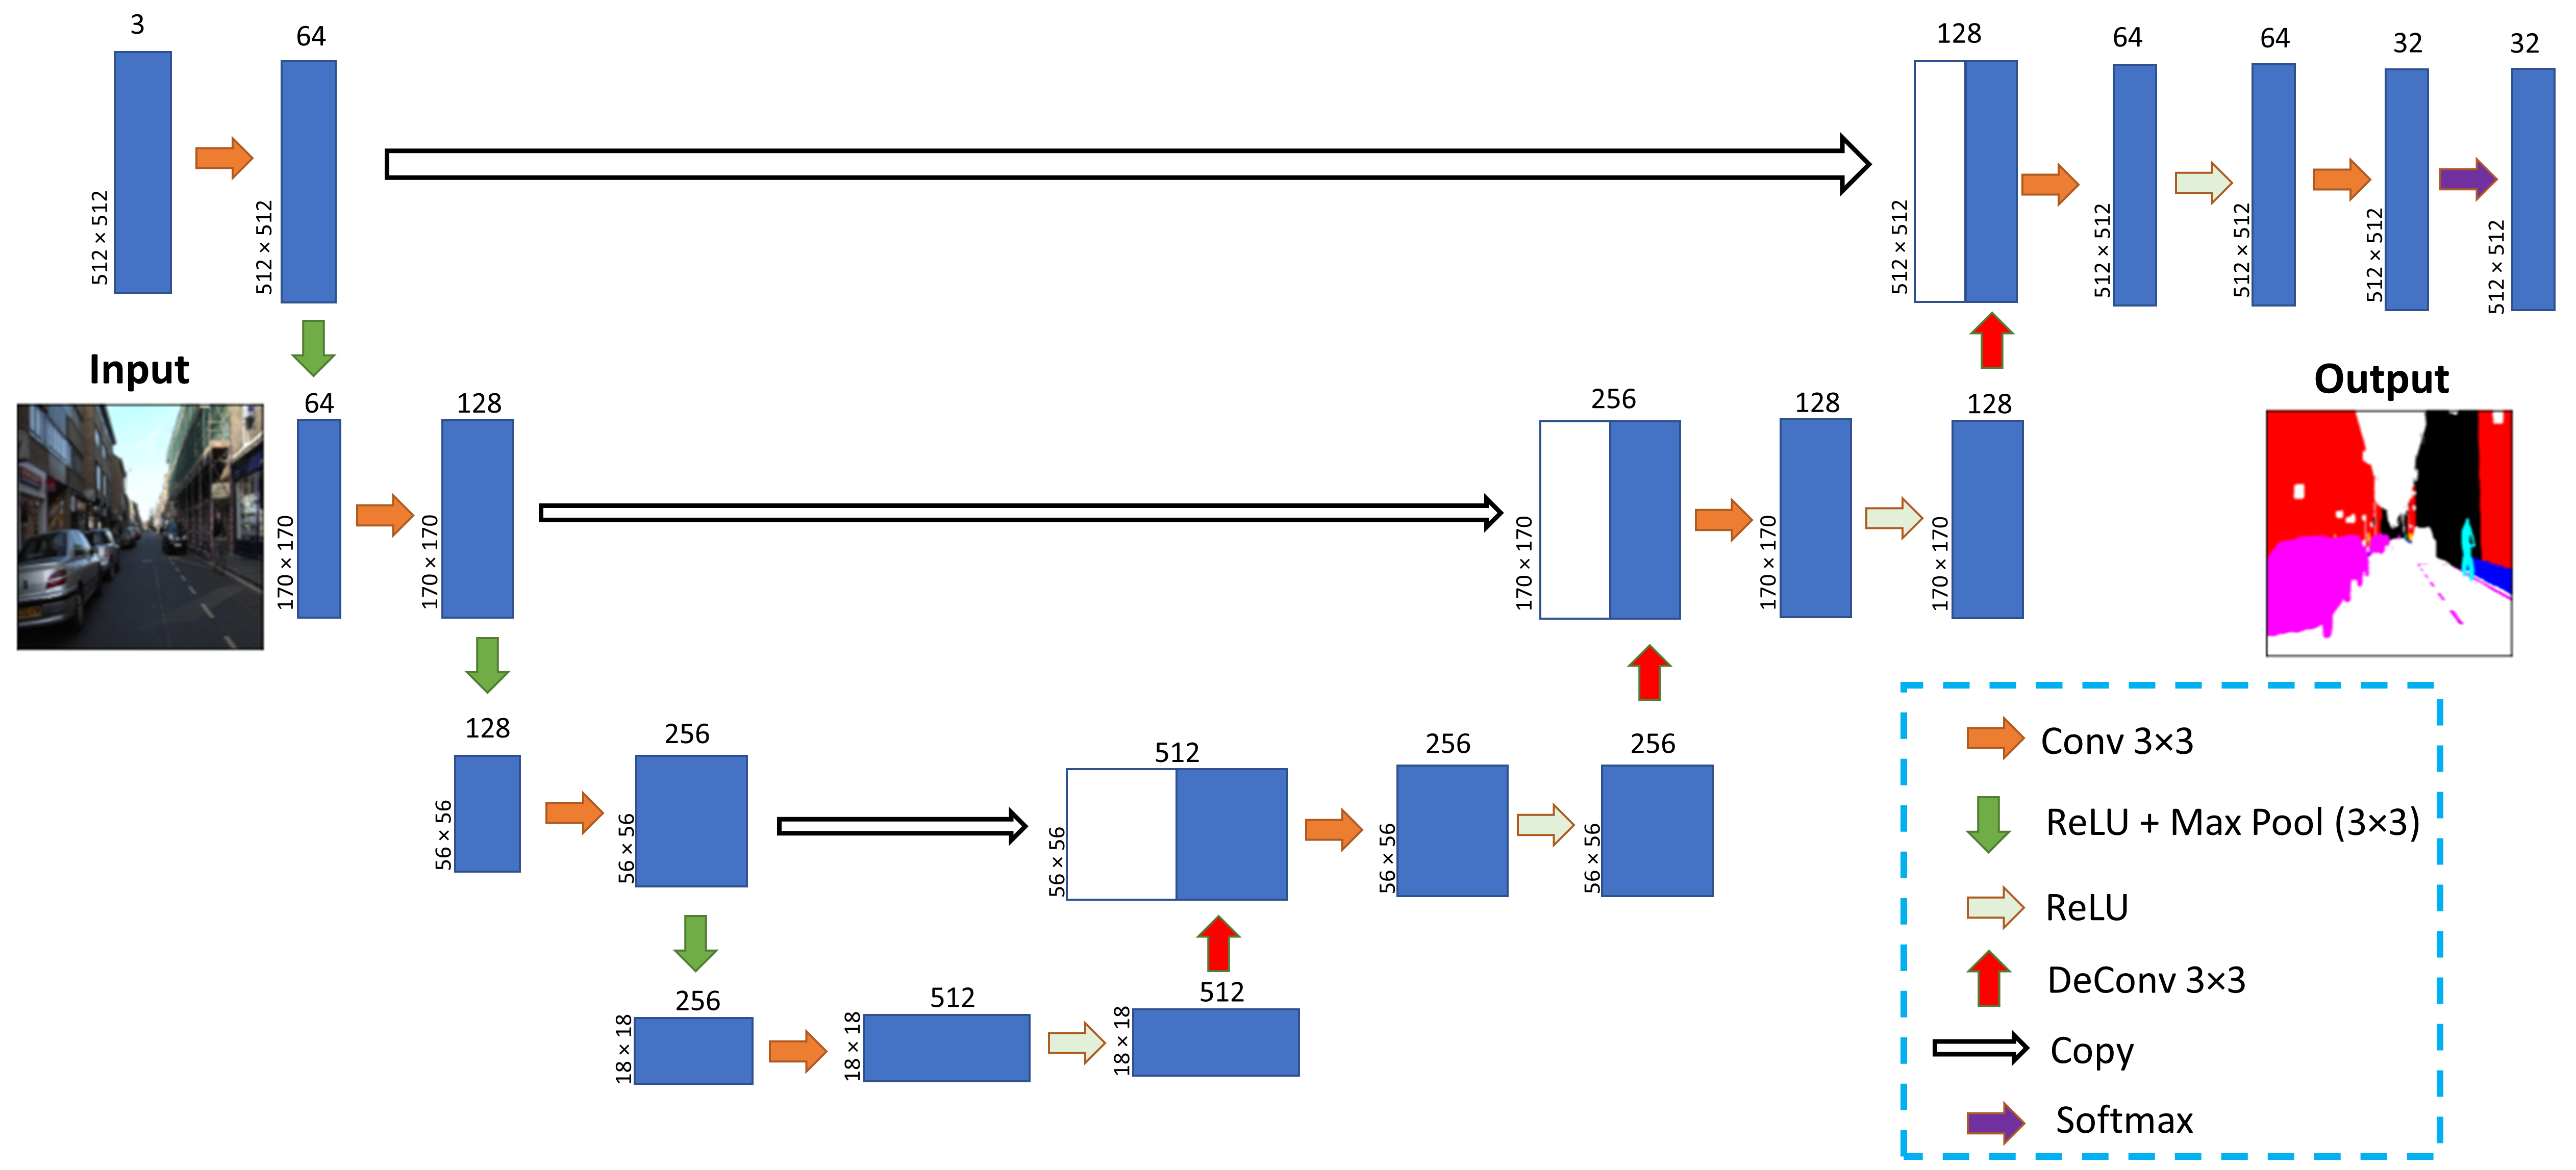
\includegraphics[width = 1\textwidth]{figures/U_Net_arch.png}
    \end{figure}
\end{frame}

\begin{frame}{}{Loss Functions}
    3 main loss functions are used for image segmentation tasks:
    \begin{itemize}
        \item \textbf{Categorical Cross-Entropy Loss:} Used for multi-class segmentation tasks where each pixel is classified into one of multiple classes.
              \only<2>{
              $$\mathcal{L} = -\frac{1}{N}\sum_{i=1}^{N}\sum_{c=1}^{C}y_{i,c}\log(\hat{y}_{i,c})$$
              }
        \item \textbf{Dice Loss:} A similarity-based loss function that measures the overlap between the predicted segmentation mask and the ground truth mask.
              \only<3>{
                  $$\mathcal{L} = 1 - \frac{2\sum_{i=1}^{N}y_i\hat{y}_i}{\sum_{i=1}^{N}y_i + \sum_{i=1}^{N}\hat{y}_i}$$
              }
        \item \textbf{Shaped aware Loss:} A loss function that penalizes the model for making errors near the object boundaries, where the segmentation is most critical.
              \only<4>{
              $$\mathcal{L} = -w(x)\left[\frac{1}{N}\sum_{i=1}^{N}\sum_{c=1}^{C}y_{i,c}\log(\hat{y}_{i,c})\right]$$
              with $w(x)$ a weight function that assigns higher weights to pixels near the object boundaries.
              }
    \end{itemize}
\end{frame}


\begin{frame}{}{The dataset}
    The dataset presented here is hosted in the BioStudies database under accession number S-BSST265 18. It consists of 79 fluorescence images of immuno and DAPI stained samples containing 7813 nuclei in total. The images are derived from one Schwann cell stroma-rich tissue (from a ganglioneuroblastoma) cryosection (10 images/2773 nuclei), seven neuroblastoma (NB) patients (19 images/931 nuclei), one Wilms patient (1 image/102 nuclei), two NB cell lines (CLB-Ma, STA-NB10) (8 images/1785 nuclei) and a human keratinocyte cell line (HaCaT) (41 images/2222 nuclei). In addition, the dataset is heterogenous in aspects such as type of preparation, imaging modality, magnification, signal-to-noise ratio and other technical aspects.
    \begin{figure}
        \centering
        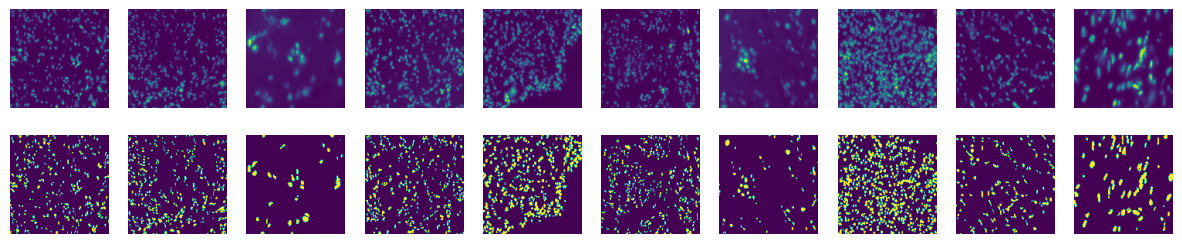
\includegraphics[width=0.8\textwidth]{figures/imagesegbio.png}
    \end{figure}
\end{frame}

% \begin{frame}{}{The U-Net Architecture}
%     U-Net is a convolutional neural network architecture designed for encoding/decoding images. It is widely used for image segmentation tasks:
%     \begin{figure}
%         \centering
%         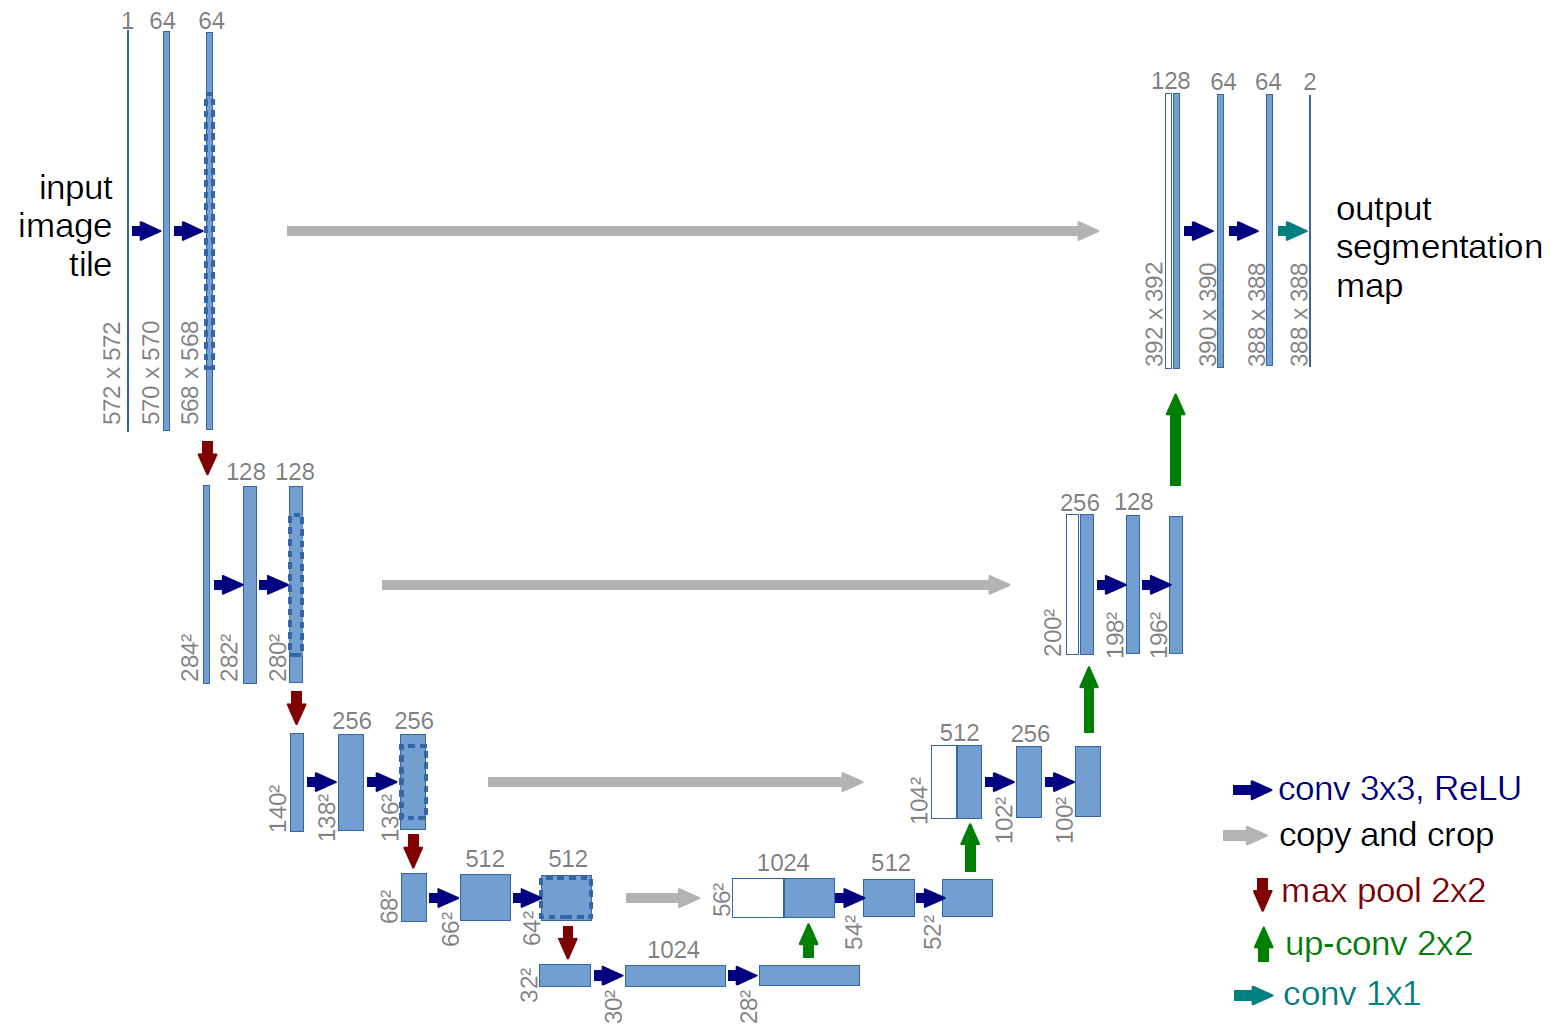
\includegraphics[width=0.7\textwidth]{figures/u-net-architecture.png}
%     \end{figure}
% \end{frame}


\subsection{Evaluating the models}

\begin{frame}
    In this example, the model is trained with the Binary Cross-Entropy loss function. Each pixel $y_{i,j}$is a label in $\{0, 1\}$, where $0$ represents the background and $1$ represents the object. The loss function is defined as:
    \[
        \text{BCE}(y, \hat{y}) = -\frac{1}{N^2} \sum_{i=1}^{N}\sum_{j=1}^{N} y_{i,j} \log(\hat{y}_{i,j}) + (1 - y_{i,j}) \log(1 - \hat{y}_{i,j})
    \]
    where $N$ is the number of pixels in the image, $y$ is the ground truth mask, and $\hat{y}$ is the predicted mask. The BCE loss function is used to measure the pixel-wise binary classification error between the ground truth and the predicted mask.
    \vspace{0.5cm}
    \textbf{Question:} What can we use to evaluate the performance of the model?
\end{frame}

\begin{frame}{}{Interpreting the output}
    The first metrics that comes to mind is cross-entropy on the test set. However, it is not the best metric to evaluate the performance of a segmentation model. The reason is that the model predicts probabilities for each pixel, and the thresholding of these probabilities is not taken into account in the BCE loss.\\
    \vspace{1cm}
    The model predicts values in $\mathbb{R}$ for each pixel. We can use a threshold to binarize the predictions:
    \vfill
    \begin{figure}
        \centering
        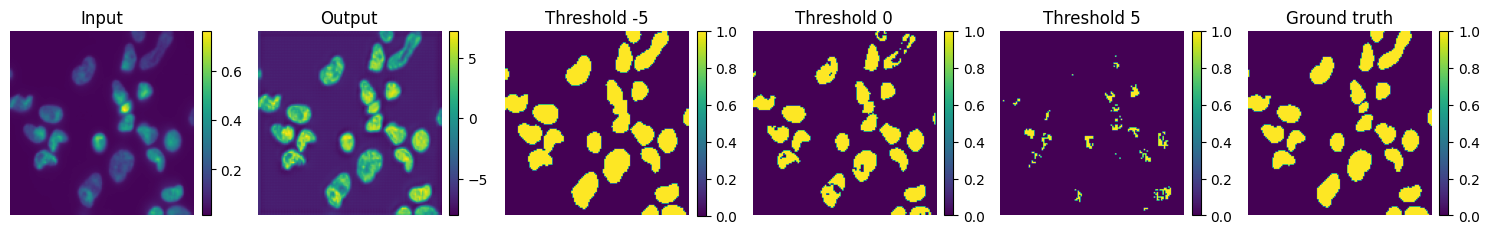
\includegraphics[width=1\textwidth]{figures/outputs.png}
    \end{figure}

\end{frame}

\begin{frame}[t]{}{The Accuracy}
    The accuracy is a common metric used to evaluate the performance of classification models. The accuracy is defined as:
    \[
        \text{Accuracy} = \frac{\text{Number of correct predictions}}{\text{Total number of predictions}}
    \]
    \vfill
    \begin{figure}
        \centering
        \only<1>{
            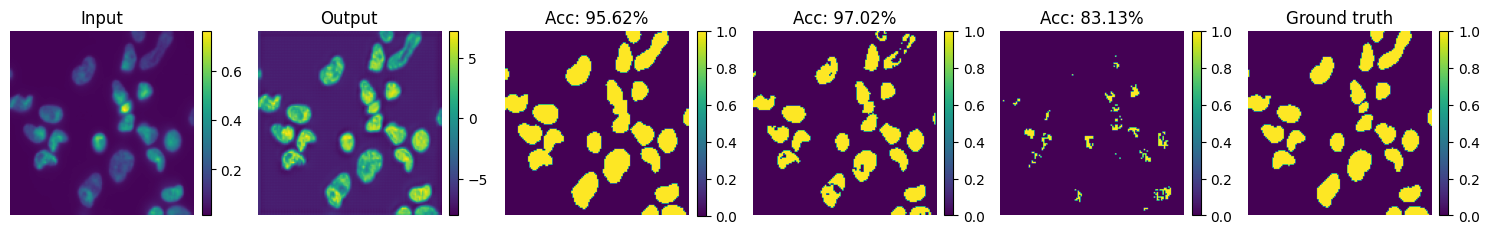
\includegraphics[width=0.9\textwidth]{figures/accs.png}}
        \only<2>{
            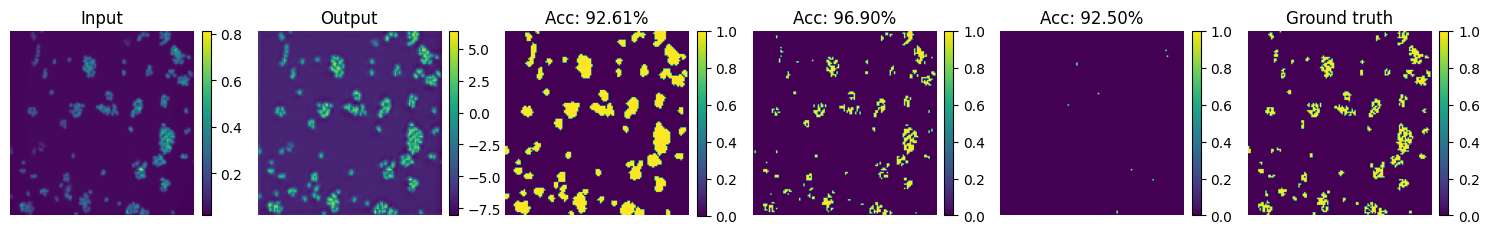
\includegraphics[width=0.9\textwidth]{figures/accs2.png}}
    \end{figure}
    \only<2>{However, missing a label $0$ is not the same as missing a label $1$ ! }
\end{frame}

\begin{frame}{}{Confusion Matrix}
    The confusion matrix is a useful tool for evaluating classification models, particularly for segmentation. It helps to distinguish between different types of errors.

    \vfill
    \begin{columns}
        \column{0.4\textwidth}
        \begin{itemize}
            \item \textbf{True Positives (TP)}: \\Correctly predicted positives.
            \item \textbf{False Positives (FP)}: \\Incorrectly predicted positives.
            \item \textbf{False Negatives (FN)}: \\Missed positives.
            \item \textbf{True Negatives (TN)}: \\Correctly predicted negatives.
        \end{itemize}

        \column{0.6\textwidth}
        \centering
        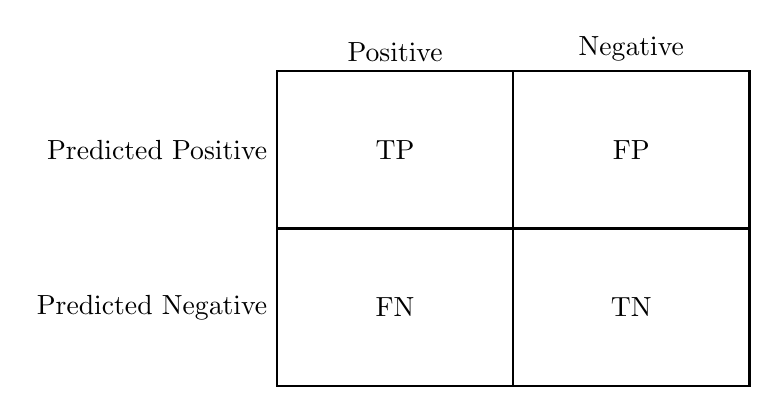
\begin{tikzpicture}
            \draw[thick] (0,0) rectangle (6,4);

            % Grid lines
            \draw[thick] (3,0) -- (3,4);
            \draw[thick] (0,2) -- (6,2);

            % Labels
            \node[anchor=south] at (1.5,4) {Positive};
            \node[anchor=south] at (4.5,4) {Negative};
            \node[anchor=east] at (0,3) {Predicted Positive};
            \node[anchor=east] at (0,1) {Predicted Negative};

            % Matrix Entries
            \node at (1.5,3) {TP};
            \node at (4.5,3) {FP};
            \node at (1.5,1) {FN};
            \node at (4.5,1) {TN};
        \end{tikzpicture}
    \end{columns}
\end{frame}

\begin{frame}{}{Precision and Recall}
    \begin{columns}

        \column{0.6\textwidth}
        \centering
        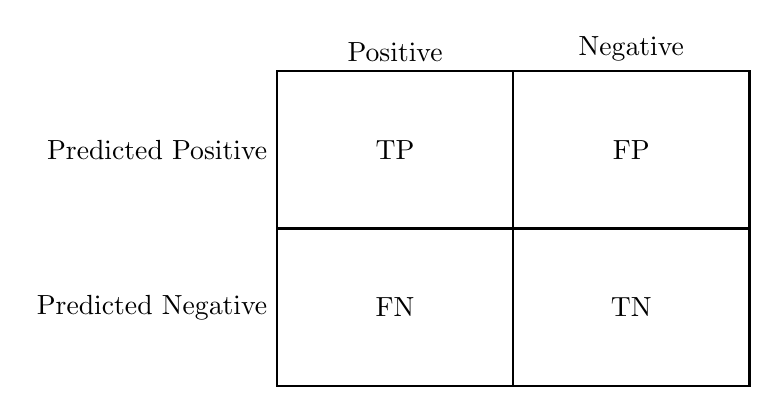
\begin{tikzpicture}
            \draw[thick] (0,0) rectangle (6,4);

            % Grid lines
            \draw[thick] (3,0) -- (3,4);
            \draw[thick] (0,2) -- (6,2);

            % Labels
            \node[anchor=south] at (1.5,4) {Positive};
            \node[anchor=south] at (4.5,4) {Negative};
            \node[anchor=east] at (0,3) {Predicted Positive};
            \node[anchor=east] at (0,1) {Predicted Negative};

            % Matrix Entries
            \node at (1.5,3) {TP};
            \node at (4.5,3) {FP};
            \node at (1.5,1) {FN};
            \node at (4.5,1) {TN};
        \end{tikzpicture}
        \column{0.4\textwidth}
        To evaluate the performance of a segmentation model, we can use the following metrics:
        \begin{align*}
            \mathrm{Accuracy} & = \frac{TP + TN}{P + N}
        \end{align*}
        \begin{align*}
            \mathrm{Precision} & = \frac{TP}{TP + FP}
        \end{align*}
        \begin{align*}
            \mathrm{Recall} & = \frac{TP}{P}
        \end{align*}
    \end{columns}

\end{frame}

\begin{frame}{}{Confusion Matrix}
    Examples with a cancer detection model with 100 patients (20 with cancer and 80 without cancer):
    \begin{center}
        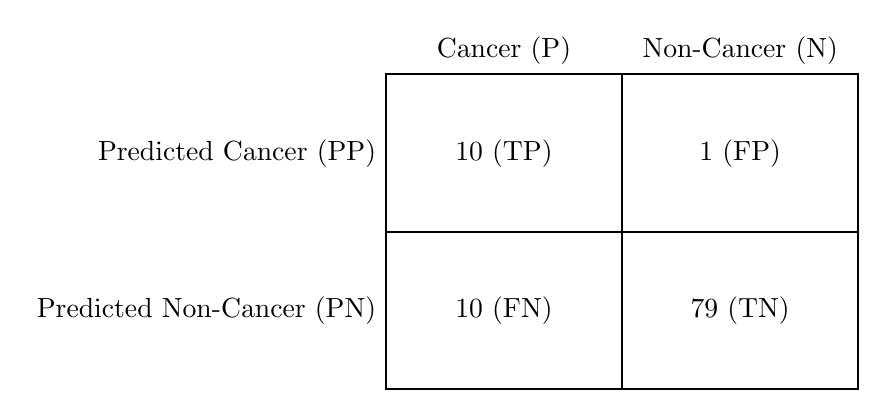
\begin{tikzpicture}
            \draw[thick] (0,0) rectangle (6,4);

            % Grid lines
            \draw[thick] (3,0) -- (3,4);
            \draw[thick] (0,2) -- (6,2);

            % Labels
            \node[anchor=south] at (1.5,4) {Cancer (P)};
            \node[anchor=south] at (4.5,4) {Non-Cancer (N)};
            \node[anchor=east] at (0,3) {Predicted Cancer (PP)};
            \node[anchor=east] at (0,1) {Predicted Non-Cancer (PN)};

            % Matrix Entries
            \node at (1.5,3) {10 (TP)};
            \node at (4.5,3) {1 (FP)};
            \node at (1.5,1) {10 (FN)};
            \node at (4.5,1) {79 (TN)};
        \end{tikzpicture}
        \\
        \vspace{1cm}
        Accuracy: $\frac{TP + TN}{P + N} = \frac{10 + 79}{20 + 80} = 0.89\quad$  Precision: $\frac{TP}{TP + FP} = \frac{10}{10 + 1} = 0.90\quad$ Recall: $\frac{TP}{P} = \frac{10}{20} = 0.5$
    \end{center}
\end{frame}

\begin{frame}{}{Confusion Matrix}
    Examples with a financial operation models with 100 operations (20 high reward and 80 high loss):
    \begin{center}
        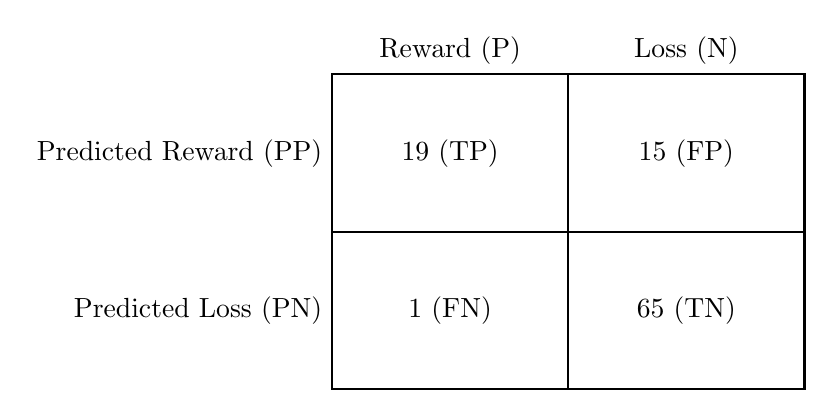
\begin{tikzpicture}
            \draw[thick] (0,0) rectangle (6,4);

            % Grid lines
            \draw[thick] (3,0) -- (3,4);
            \draw[thick] (0,2) -- (6,2);

            % Labels
            \node[anchor=south] at (1.5,4) {Reward (P)};
            \node[anchor=south] at (4.5,4) {Loss (N)};
            \node[anchor=east] at (0,3) {Predicted Reward (PP)};
            \node[anchor=east] at (0,1) {Predicted Loss (PN)};

            % Matrix Entries
            \node at (1.5,3) {19 (TP)};
            \node at (4.5,3) {15 (FP)};
            \node at (1.5,1) {1 (FN)};
            \node at (4.5,1) {65 (TN)};
        \end{tikzpicture}
        \\
        \vspace{1cm}
        Accuracy: $\frac{TP + TN}{P + N} = \frac{19 + 65}{20 + 80} = 0.84\quad$  Precision: $\frac{TP}{TP + FP} = \frac{19}{19 + 15} = 0.56\quad$ Recall: $\frac{TP}{P} = \frac{19}{20} = 0.95$
    \end{center}
\end{frame}


\begin{frame}{}{Precision-Recall Curve}
    In Image segmentation tasks, by adjusting the threshold we can change the precision and recall of the model. The Precision-Recall curve is a useful tool to evaluate the performance of a model across different thresholds:
    \begin{figure}
        \centering
        \only<1>{
            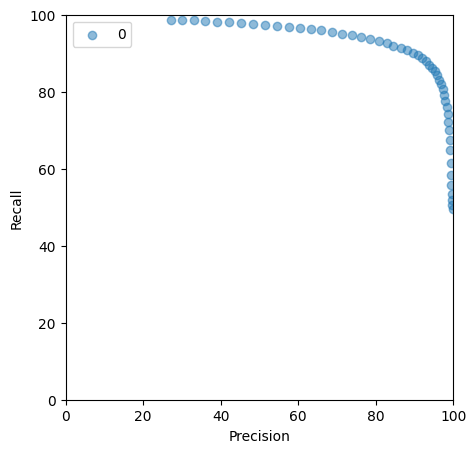
\includegraphics[width=0.5\textwidth]{figures/prcurve.png}}
        \only<2>{
            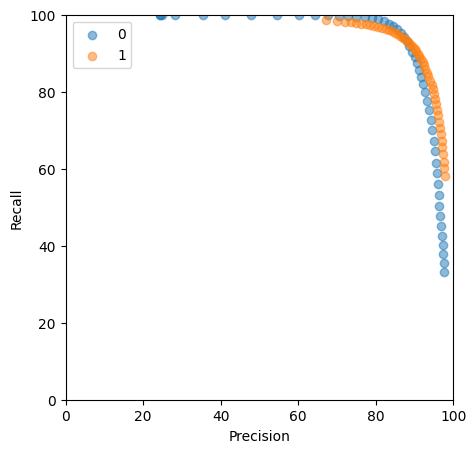
\includegraphics[width=0.5\textwidth]{figures/prcurve2.png}}
    \end{figure}
\end{frame}

\begin{frame}{}{Your turn !}
    Get the Notebook on the course website and start working on it.
    \begin{itemize}
        \item \url{https://www.alexverine.com}
        \item Teaching
        \item Introduction to Deep Learning
        \item Lien Notebook
    \end{itemize}
    During this hands-on session we will compare the speed of the model with and without the GPU, and we will evaluate the model with the metrics we have seen. Don't hesitate to use Colab or your own computer to run the notebook.
\end{frame}



\section{Synthetic Data Generation with Generative Adversarial Networks}
\subsection{GANS Models}
\begin{frame}
    Generative Adversarial Networks (GANs) are a type of deep learning architecture composed of two neural networks, the generator and the discriminator, that are trained in a adversarial manner. The generator network is trained to generate fake data that appears similar to real data, while the discriminator network is trained to distinguish between real and fake data. The loss for GANs is defined as a min-max game, where the generator minimizes the loss function, and the discriminator maximizes it. $D$ and $G$ represent the discriminator and generator networks, respectively, and the goal is to find the optimal configuration for $D$ and $G$ such that the generated samples appear indistinguishable from real data.

    \begin{figure}
        \centering
        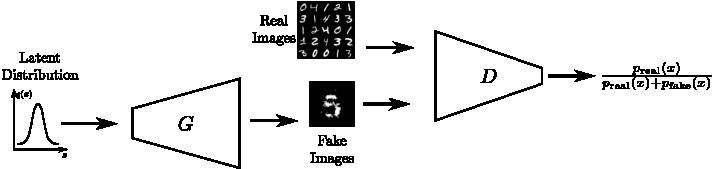
\includegraphics[width = 0.9\textwidth]{figures/GAN.pdf}
    \end{figure}
\end{frame}
\begin{frame}
    The loss of a  (GAN) is defined as a minimax game between the generator and discriminator models. The generator aims to generate samples that are indistinguishable from real samples, while the discriminator aims to distinguish the generated samples from real samples. The loss function for the generator is defined as $-\log(D(G(z)))$, where $D$ is the discriminator model and $G(z)$ is the generator's output for a random noise vector $z$. The loss function for the discriminator is defined as $\log(D(x)) + \log(1 - D(G(z)))$, where $x$ is a real sample.
    $$
        \min_D \max_G \mathbb{E}_{x\sim p_{\mathrm{real}}}\left[\log(D(x))\right]  +  \mathbb{E}_{z\sim q}\left[ \log(1 - D(G(z)))\right]
    $$

    \begin{figure}
        \centering
        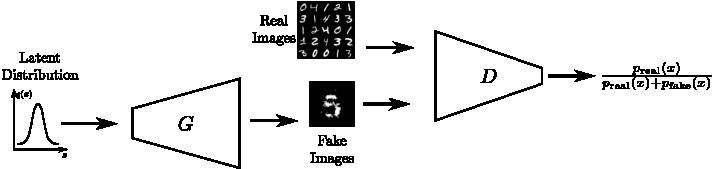
\includegraphics[width = 0.9\textwidth]{figures/GAN.pdf}
    \end{figure}
\end{frame}

% --- SLIDE 1 ---
\begin{frame}{Generative Adversarial Networks (GANs)}{Intro: year, reference, roles of D \& G}
    \textbf{Introduced in:} 2014a by \citet{goodfellow_generative_2014}.\\
    \medskip
    \begin{itemize}
        \item \textbf{Discriminator $D(x)$}: estimates how likely a sample $x$ is \emph{real} (vs. generated).
        \item \textbf{Generator $G(z)$}: maps noise $z\sim Q$ to data space and aims to \emph{fool} $D$.
    \end{itemize}
    \begin{figure}
        \centering
        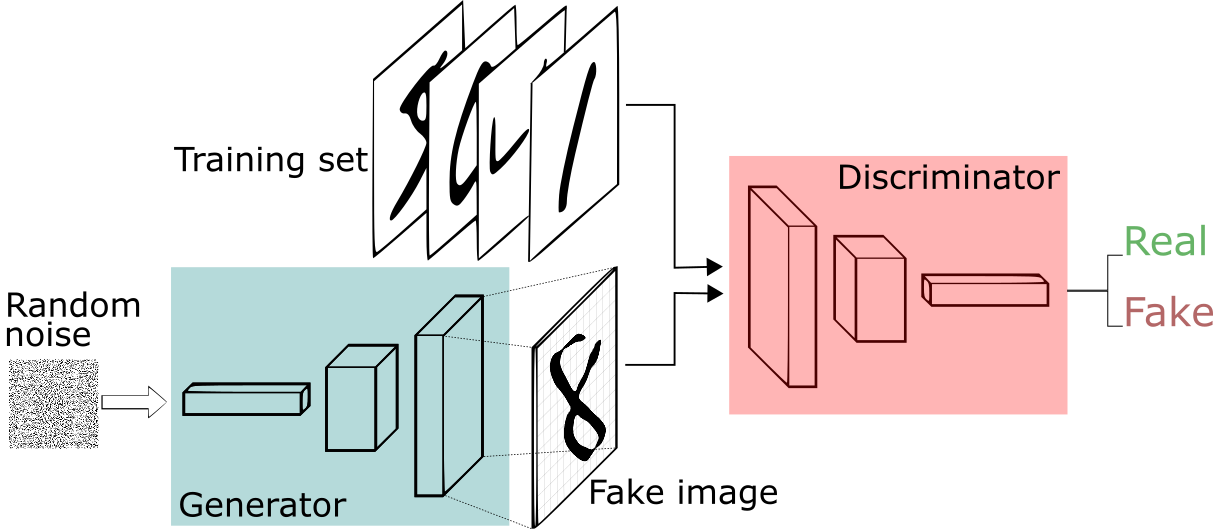
\includegraphics[width=0.8\textwidth]{figures/GANs.png}
    \end{figure}
\end{frame}

% --- SLIDE 1.5.1 ---
\begin{frame}[t]{Training the Discriminator as a Classifier}{Labels, loss selection, BCE/logistic}
    \only<1->{
        \textbf{Setup:} assign labels $y\in\{-1, +1\}$ with $y=+1$ for real $x\sim P$ and $y=-1$ for fake $x\sim \widehat{P}$.\\
        \textbf{Goal:} Train a classifier parametrized by $D=\sigma(F_\theta)$ to distinguish real vs fake.\\
        \medskip
        \textbf{Question:} which loss to train $D$ as a classifier?
    }

\end{frame}

% Replace frame title and subtitle as requested
\begin{frame}{Sigmoid and Logit}{Activation \& link functions}
    \begin{itemize}
        \item The \textbf{sigmoid function} $\sigma:\mathbb{R}\to[0,1]$ is defined as:
              \begin{equation}
                  \sigma(x) = \frac{1}{1+\exp(-x)}.
              \end{equation}
        \item It maps any real-valued number $x$ to the interval $[0,1]$, suitable for modeling probabilities.
        \item The \textbf{logit function} $\text{logit}:[0,1]\to\mathbb{R}$ is defined as the inverse of the sigmoid:
              \begin{equation}
                  \text{logit}(p) = \log\left(\frac{p}{1-p}\right).
              \end{equation}
        \item Let $D(x) = \sigma(F_\theta(x))$ be a discriminator outputting probabilities. We call $F_\theta(x)$ the \textbf{logit} of $D$ and $D(x)$ the \textbf{probit}.
    \end{itemize}
    \medskip
    \begin{figure}
        \centering
        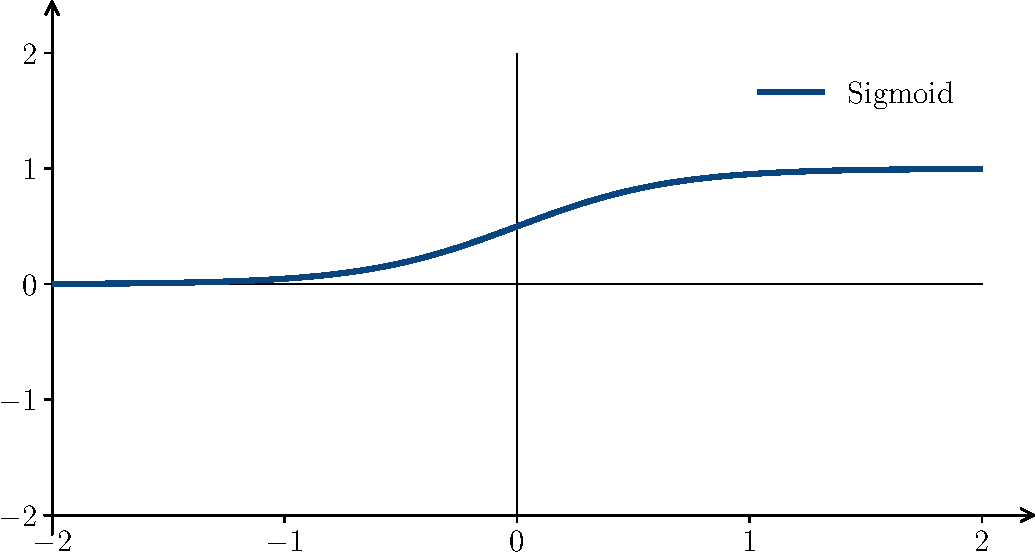
\includegraphics[width=0.35\textwidth]{figures/sigmoid.pdf}
        \caption{Sigmoid function mapping logits to probabilities.}
    \end{figure}
\end{frame}


% --- SLIDE 1.5.1 ---
\begin{frame}[t]{Training the Discriminator as a Classifier}{Question → Answer → Loss decomposition}
    \only<1->{
        \textbf{Setup:} assign labels $y\in\{-1, +1\}$ with $y=+1$ for real $x\sim P$ and $y=-1$ for fake $x\sim \widehat{P}$.\\
        \textbf{Goal:} Train a classifier parametrized by $D=\sigma(F_\theta)$ to distinguish real vs fake.\\
        \medskip
        \only<1>{
            \textbf{Question:} which loss to train $D$ as a classifier?}
    }
    \only<2->{
        \textbf{Answer:} binary cross-entropy / logistic loss (with logits).\\
    }
    \only<3->{
        \textbf{Loss with labels:}
        \begin{equation*}
            \mathcal{L}_D = \mathbb{E}_{(x,y)}\Big[\log\big(1+\exp(-y\, F_\theta(x))\big)\Big].
        \end{equation*}
        \textbf{Decomposition over $P$ and $\widehat{P}$:}
        \begin{align*}
            \mathcal{L}_D & = \mathbb{E}_{x\sim P}\big[\log(1+\exp(-F_\theta(x)))\big]
            \quad + \mathbb{E}_{x\sim \widehat{P}}\big[\log(1+\exp(F_\theta(x)))\big]                                                                                                                          \\
                          & =\mathbb{E}_{x\sim P}\big[- \log \left(\frac{1}{1+\exp(-F_\theta(x))}\right)\big] + \mathbb{E}_{x\sim \widehat{P}}\big[- \log \left(1 - \frac{1}{1+\exp(-F_\theta(x))}\right)\big] \\
                          & = -\mathbb{E}_{x\sim P}[\log \sigma(F_\theta(x))] - \mathbb{E}_{x\sim \widehat{P}}[\log(1-\sigma(F_\theta(x)))]                                                                    \\
                          & = -\mathbb{E}_{x\sim P}[\log D(x)] - \mathbb{E}_{x\sim \widehat{P}}[\log(1-D(x))].
        \end{align*}
        \only<4>{
            Summarizing:
            \begin{equation*}
                \boxed{\text{Minimizing }\mathcal{L}_D = -\mathbb{E}_{x\sim P}[\log D(x)] - \mathbb{E}_{x\sim \widehat{P}}[\log(1-D(x))].}
            \end{equation*}}
        \only<5>{
            Summarizing:
            \begin{equation*}
                \boxed{\text{Maximizing }\mathcal{L}_D = \mathbb{E}_{x\sim P}[\log D(x)] + \mathbb{E}_{x\sim \widehat{P}}[\log(1-D(x))].}
            \end{equation*}}
    }
\end{frame}


% --- SLIDE 1.5.2 ---
\begin{frame}[t]{Training the Generator}{Minimax vs non-saturating objectives}
    \only<1->{
        \textbf{Goal:} decrease $D$'s confidence on $\widehat{P}$ (make fakes look real).
    }
    \only<2>{
        \begin{equation*}
            \boxed{\text{Maximizing }  \mathcal{L}_G = - \mathbb{E}_{x\sim \widehat{P}}[\log(1-D(x))]}
        \end{equation*}
    }
    \only<3>{
        \begin{equation*}
            \boxed{\text{Maximizing }  \mathcal{L}_G = - \mathbb{E}_{z\sim Q}[\log(1-D(G(z)))]}
        \end{equation*}
    }
    \only<4->{
        \begin{equation*}
            \boxed{\text{Minimizing }  \mathcal{L}_G = \mathbb{E}_{z\sim Q}[\log(1-D((G(z))))]}
        \end{equation*}
    }
    \only<5>{
        \textbf{Minimax formulation:} combine both objectives:
        \begin{equation*}
            \min_G \max_D\ \mathbb{E}_{x\sim P}[\log D(x)] + \mathbb{E}_{z\sim Q}[\log(1-D(G(z)))]
        \end{equation*}
    }
\end{frame}

% --- SLIDE 2 ---
\begin{frame}{Original GAN: Figures}{Training loop \& distributions}
    Example of generated samples during training from \citet{goodfellow_generative_2014}. In dotted black: the real data distribution, in blue the estimated probabilities from the discriminator and in green the generated distribution.
    \vskip 10pt
    \begin{minipage}[t]{0.31\textwidth}
        \begin{figure}
            \centering
            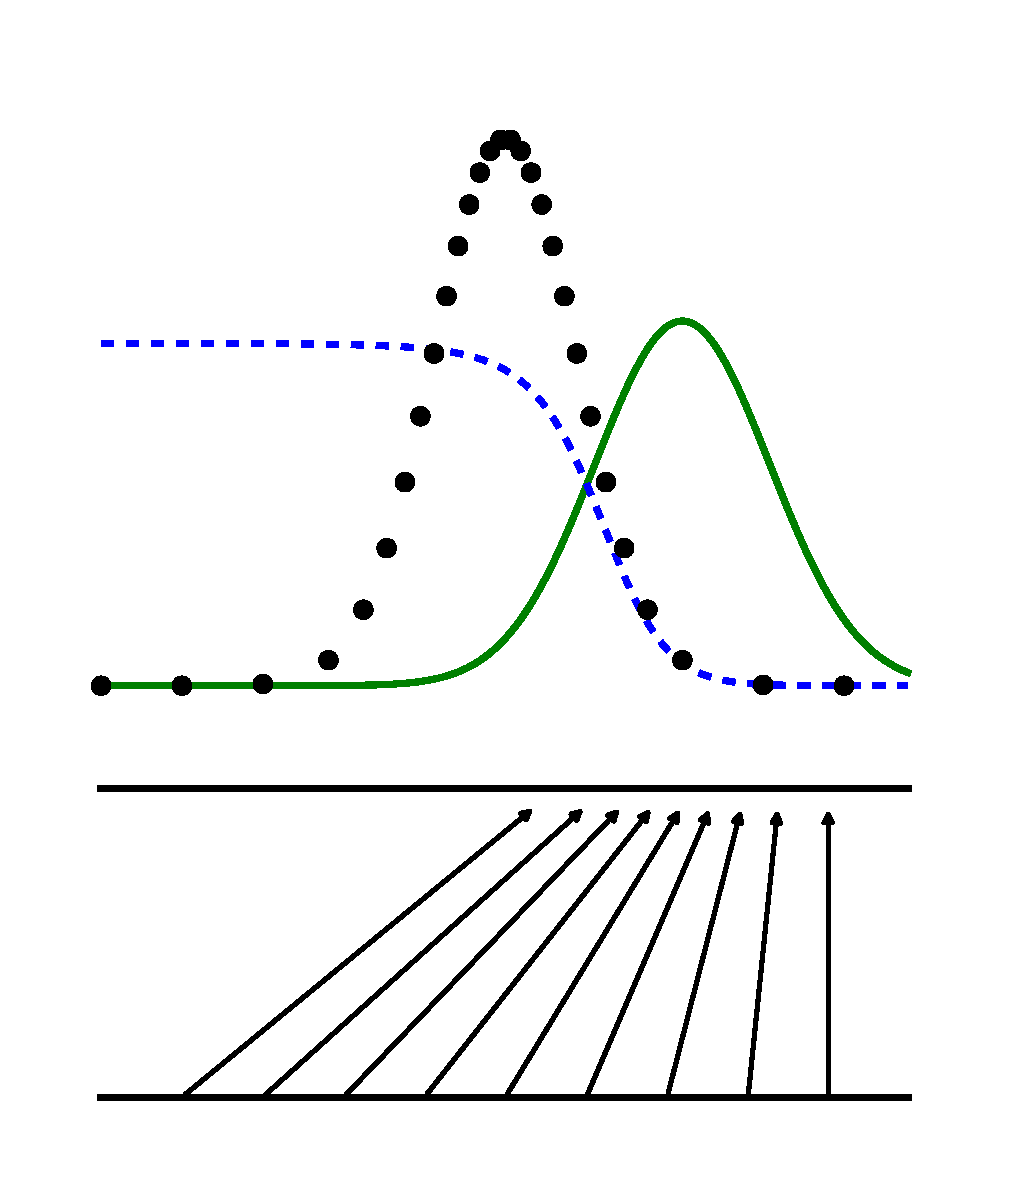
\includegraphics[width=0.9\textwidth]{figures/gan1.pdf}
            \caption{Before}
        \end{figure}
    \end{minipage}
    \hfill
    \begin{minipage}[t]{0.31\textwidth}
        \begin{figure}
            \centering
            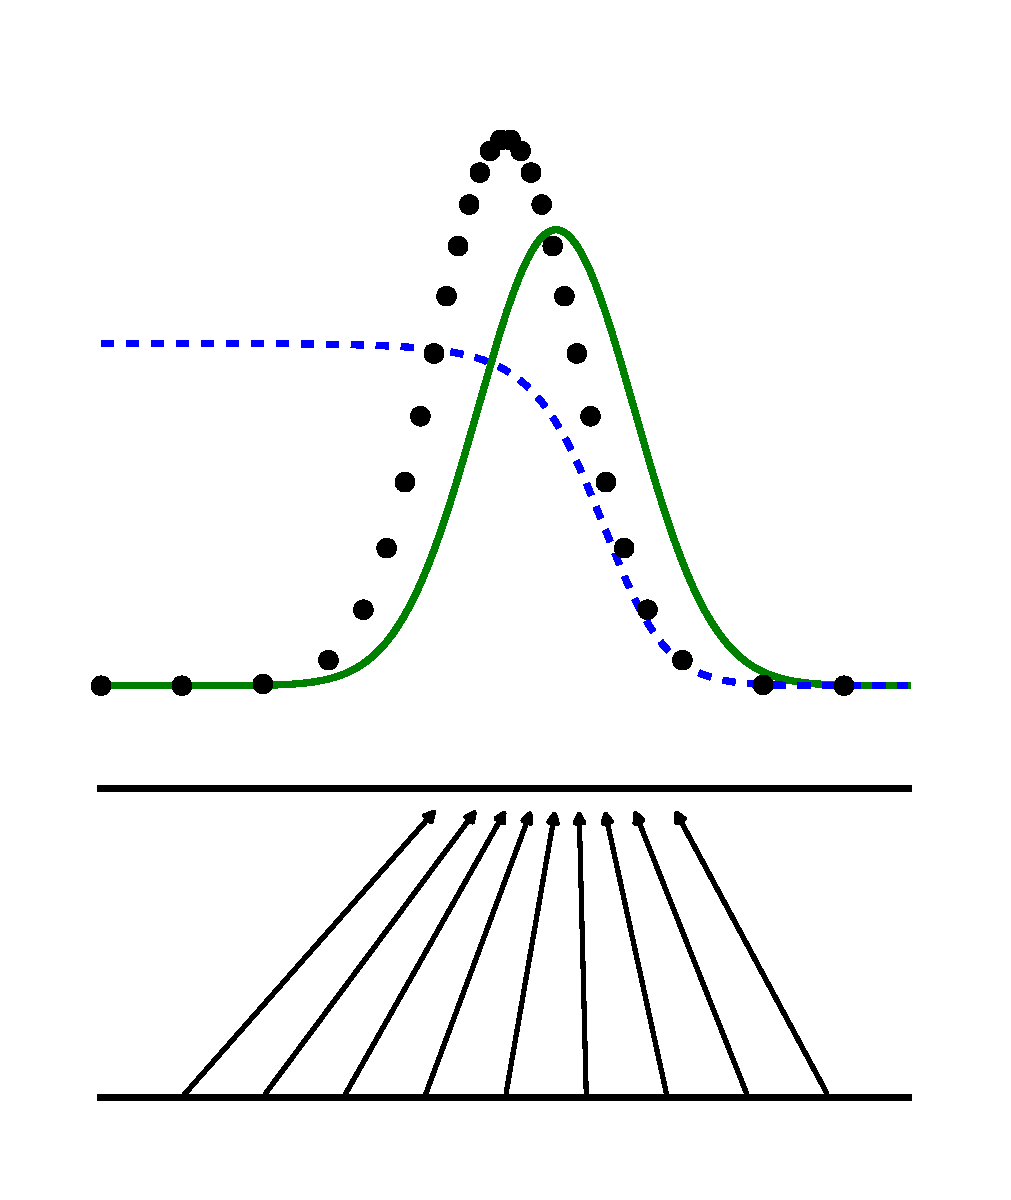
\includegraphics[width=0.9\textwidth]{figures/gan2.pdf}
            \caption{During}
        \end{figure}
    \end{minipage}
    \hfill
    \begin{minipage}[t]{0.31\textwidth}
        \begin{figure}
            \centering
            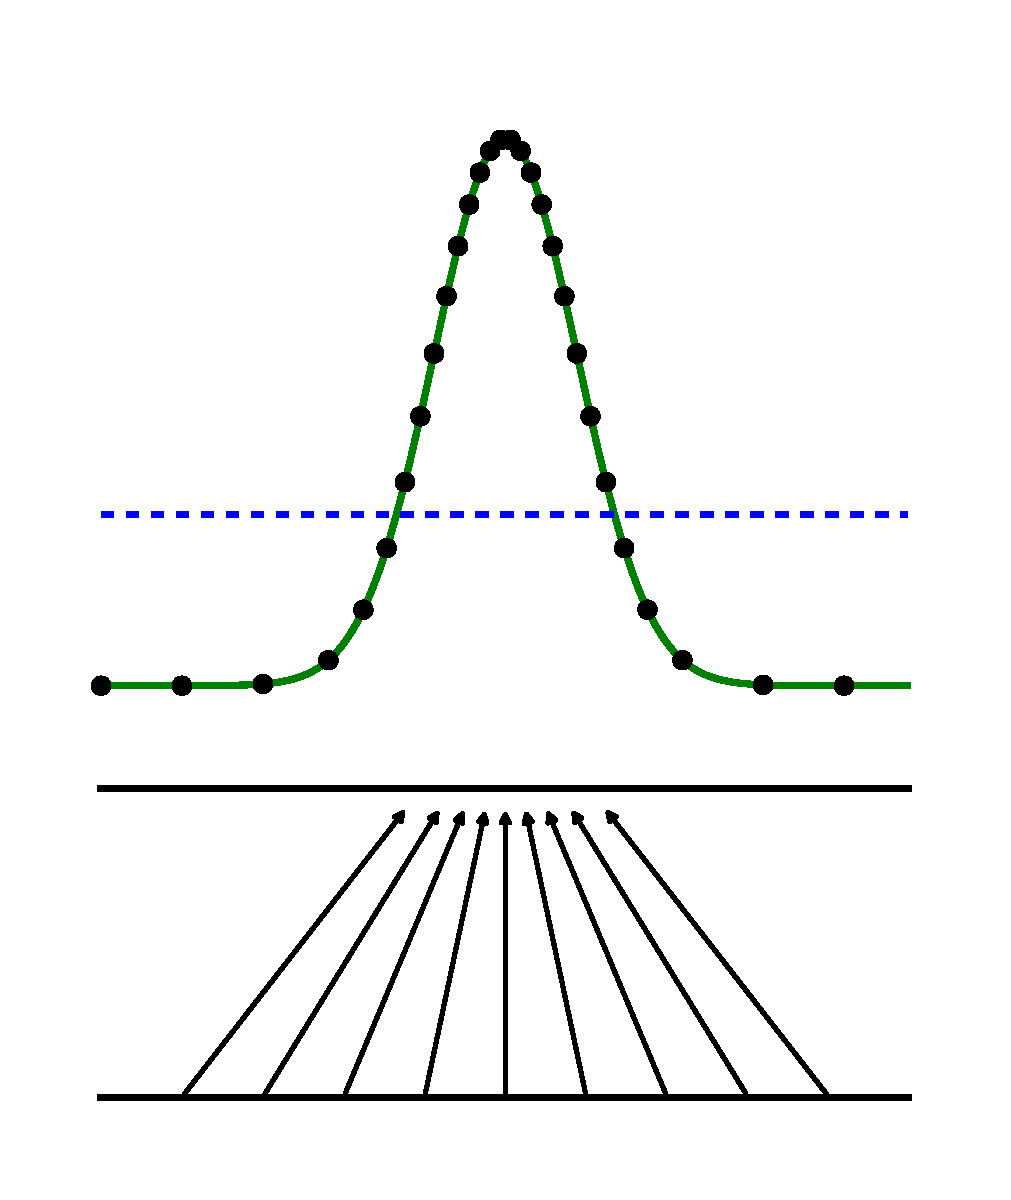
\includegraphics[width=0.9\textwidth]{figures/gan3.pdf}
            \caption{After}
        \end{figure}
    \end{minipage}

\end{frame}

% --- SLIDE 3 ---
\begin{frame}{Original GAN: Generation Examples}{Real vs generated comparisons}
    % Grid of generated samples 2x2 of MNIST, TFD, CIFAR and CIFAR with conv
    The right column shows the closest real samples to the generated ones on the left, illustrating that the model is not simply memorizing training data.\\
    \begin{minipage}[t]{0.48\textwidth}
        \begin{figure}
            \centering
            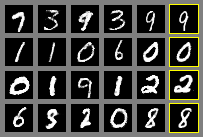
\includegraphics[width=0.5\textwidth]{figures/mnist_samples.png}
            \caption{MNIST samples}
        \end{figure}
    \end{minipage}
    \hfill
    \begin{minipage}[t]{0.48\textwidth}
        \begin{figure}
            \centering
            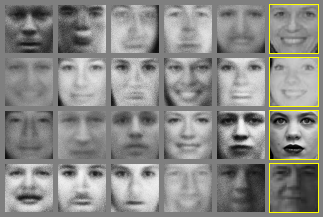
\includegraphics[width=0.5\textwidth]{figures/tfd_samples.png}
            \caption{Toronto Face Dataset samples}
        \end{figure}
    \end{minipage}
    \begin{minipage}[t]{0.48\textwidth}
        \begin{figure}
            \centering
            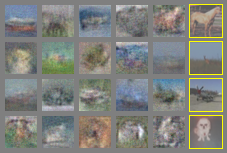
\includegraphics[width=0.5\textwidth]{figures/cifar_full_samples.png}
            \caption{CIFAR-10 samples (FC)}
        \end{figure}
    \end{minipage}
    \hfill
    \begin{minipage}[t]{0.48\textwidth}
        \begin{figure}
            \centering
            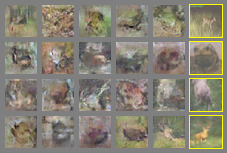
\includegraphics[width=0.5\textwidth]{figures/cifar_conv_samples.png}
            \caption{CIFAR-10 samples (ConvNet)}
        \end{figure}
    \end{minipage}
\end{frame}


\subsection{MNIST Generation}
\begin{frame}
    \begin{columns}[c, onlytextwidth]
        \column{0.5\textwidth}
        \centering $G$
        \begin{figure}
            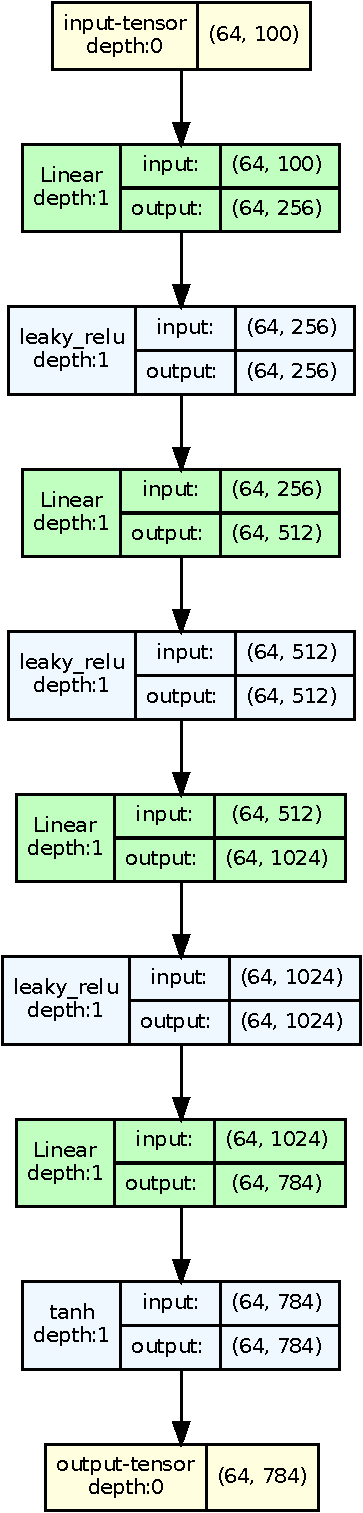
\includegraphics[width=0.2\textwidth]{figures/F.pdf}
        \end{figure}

        \column{0.5\textwidth}
        \centering $D$
        \begin{figure}
            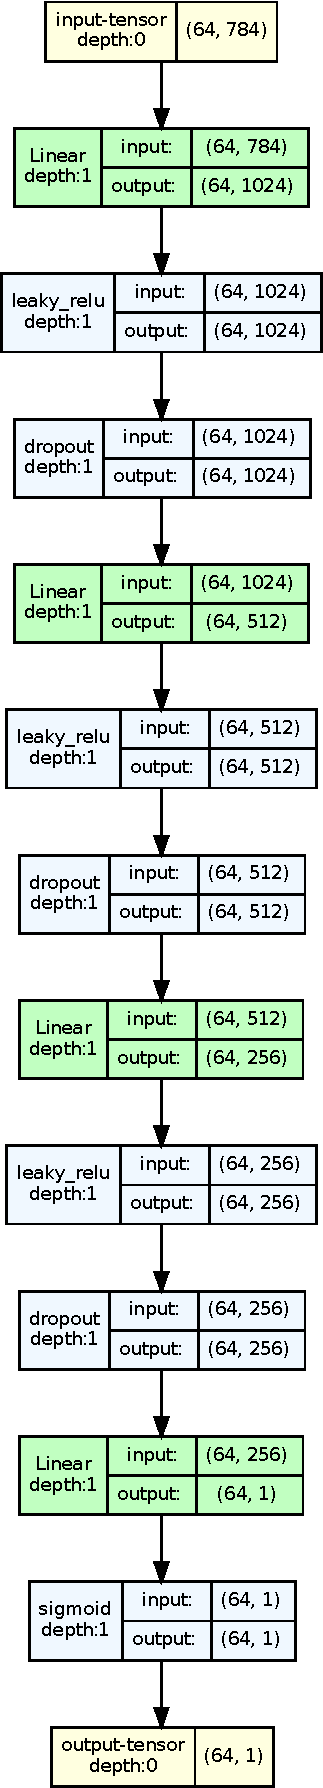
\includegraphics[width=0.2\textwidth]{figures/D.pdf}
        \end{figure}
    \end{columns}
\end{frame}

\begin{frame}
    \begin{figure}
        \centering
        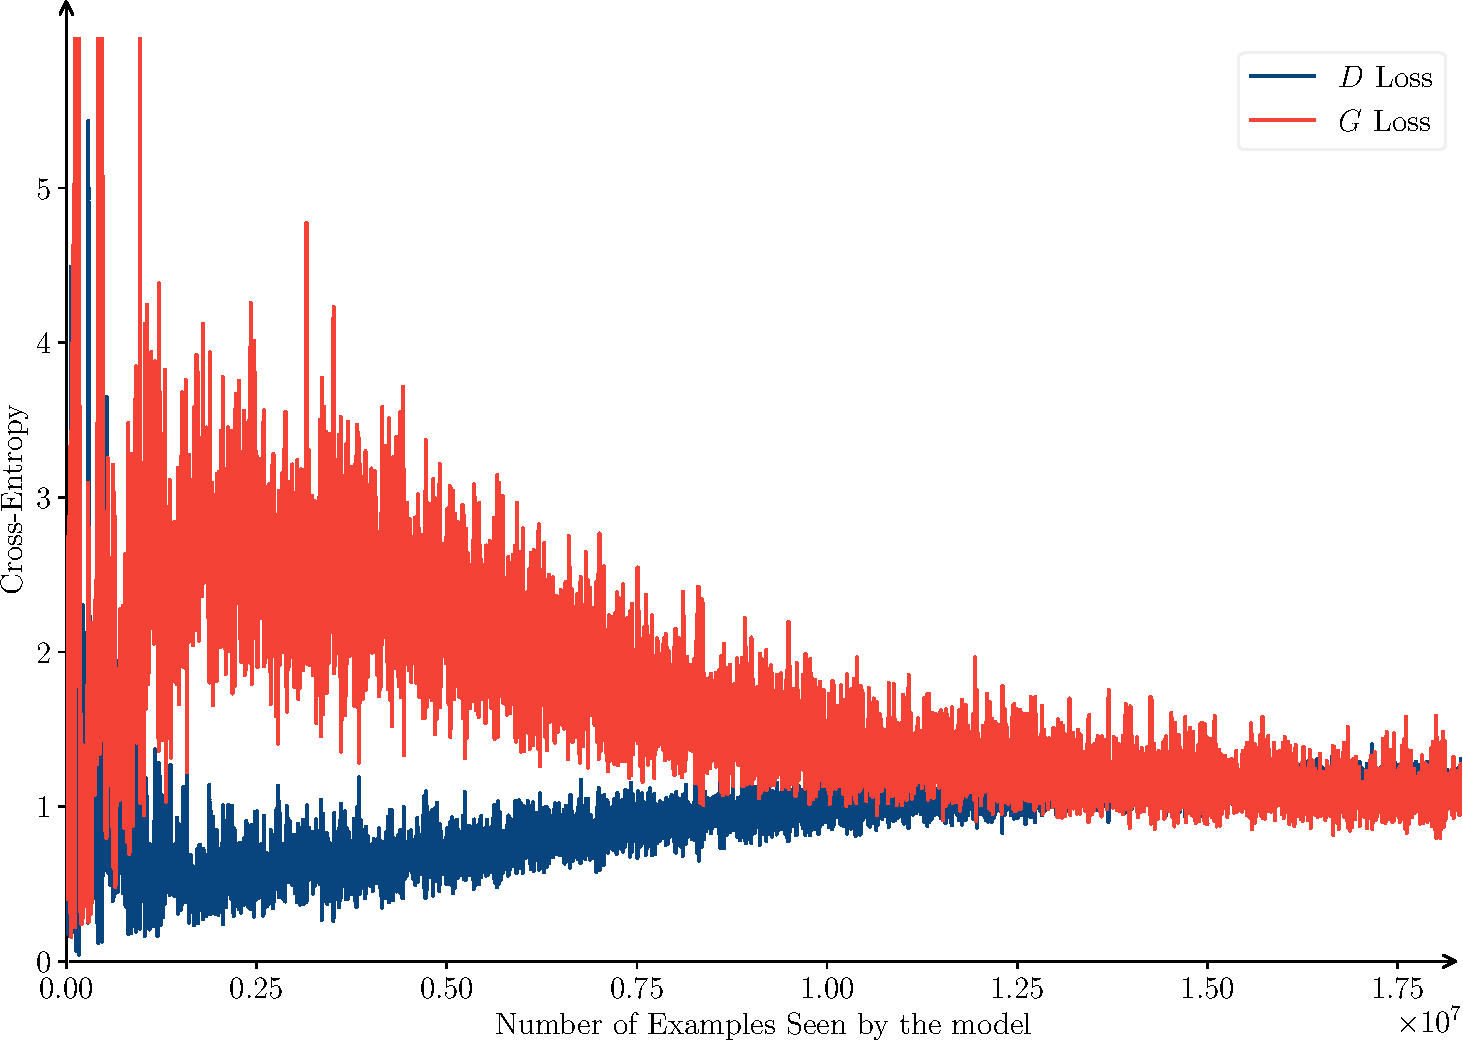
\includegraphics[width = 0.6 \textwidth]{figures/gan_loss.pdf}
    \end{figure}
\end{frame}

\begin{frame}
    \begin{figure}
        \animategraphics[autoplay,loop,width=0.4\textwidth]{15}{figures/GAN/sample_}{1}{305}
    \end{figure}
\end{frame}

% --- SLIDE 22 ---
\begin{frame}{Neural Architectures for GANs}{Why they matter \& milestones}
    \textbf{Why architectures matter}
    \begin{itemize}
        \item Stability of the adversarial game (gradient flow, Lipschitz control)
        \item Fidelity \& diversity of samples (texture, long-range structure)
        \item Scalability to high resolution and many classes
    \end{itemize}
    \vskip 6pt
    \textbf{Roadmap (milestones)}
    \begin{itemize}
        \item \textbf{2014} — Early GANs (MLPs; small images)
        \item \textbf{2015} — \emph{DCGAN}: conv/deconv stacks, BatchNorm, strided conv, (Leaky)ReLU
        \item \textbf{2017} — \emph{Progressive Growing}: fade-in layers for high-res synthesis
        \item \textbf{2018} — \emph{BigGAN}: class-conditional ResBlocks, self-attention, spectral norm
        \item \textbf{2018–2022} — \emph{StyleGAN → StyleGAN2 → StyleGAN-XL}: style modulation, noise injection, path-length reg
    \end{itemize}
    \vskip 4pt
    \textbf{Cross-cutting ideas}
    \begin{itemize}
        \item Normalization (BatchNorm in G/D; Spectral Norm in D)
        \item Conditioning (class embeddings, conditional BN)
        \item Architectural blocks (ResBlocks, attention) \& up/downsampling choices
    \end{itemize}

\end{frame}

% --- SLIDE 23 ---
\begin{frame}{Early GAN Architectures (MLP era)}{Template, limitations, takeaway}
    \textbf{Template (circa 2014)}
    \begin{itemize}
        \item \textbf{Generator $G$ (MLP):} $z\sim\mathcal N(0,I)\to$ dense layers $\to$ \texttt{tanh} output (image range $[-1,1]$)
        \item \textbf{Discriminator $D$ (MLP):} $x\to$ dense layers $\to$ sigmoid probability $D(x)\in(0,1)$
        \item Activations: ReLU/LeakyReLU in hidden layers; occasional Dropout; limited/no BN
        \item Target resolutions: small ($28\times28$, $32\times32$)
    \end{itemize}
    \vskip 6pt
    \textbf{Limitations observed}
    \begin{itemize}
        \item Poor inductive bias for images (no convolutions $\Rightarrow$ weak locality/translation handling)
        \item Training instability \& mode collapse at higher resolutions
        \item Limited long-range structure; textures often unrealistic
    \end{itemize}
    \vskip 4pt
    \textbf{Takeaway} \; Convolutional hierarchies (DCGAN) became the default to encode locality, share weights, and stabilize training.
\end{frame}

% --- SLIDE 24 ---
\begin{frame}{DCGAN}{Convolutional guidelines \& design choices}
    \textbf{Architecture guidelines for stable Deep Convolutional GANs (DCGAN) \citep{radford_unsupervised_2016}:}
    \begin{itemize}
        \item \textbf{Replace pooling} with \emph{strided convolutions} (discriminator) and \emph{fractional-strided convolutions} (generator).
        \item \textbf{Use BatchNorm} in both the generator and the discriminator.
        \item \textbf{Remove fully connected hidden layers} for deeper architectures.
        \item \textbf{Use ReLU in the generator} for all layers \textbf{except} the output, which uses \texttt{tanh}.
        \item \textbf{Use LeakyReLU in the discriminator} for \emph{all} layers.
    \end{itemize}
    \vskip 6pt
    \textit{Rationale:} encourage stable gradients, better conditioning, and convolutional inductive biases (locality, translation equivariance).
\end{frame}

% --- SLIDE 24.5 ---
\begin{frame}{DCGAN}{Architecture diagram \& rules of thumb}
    \begin{figure}
        \centering
        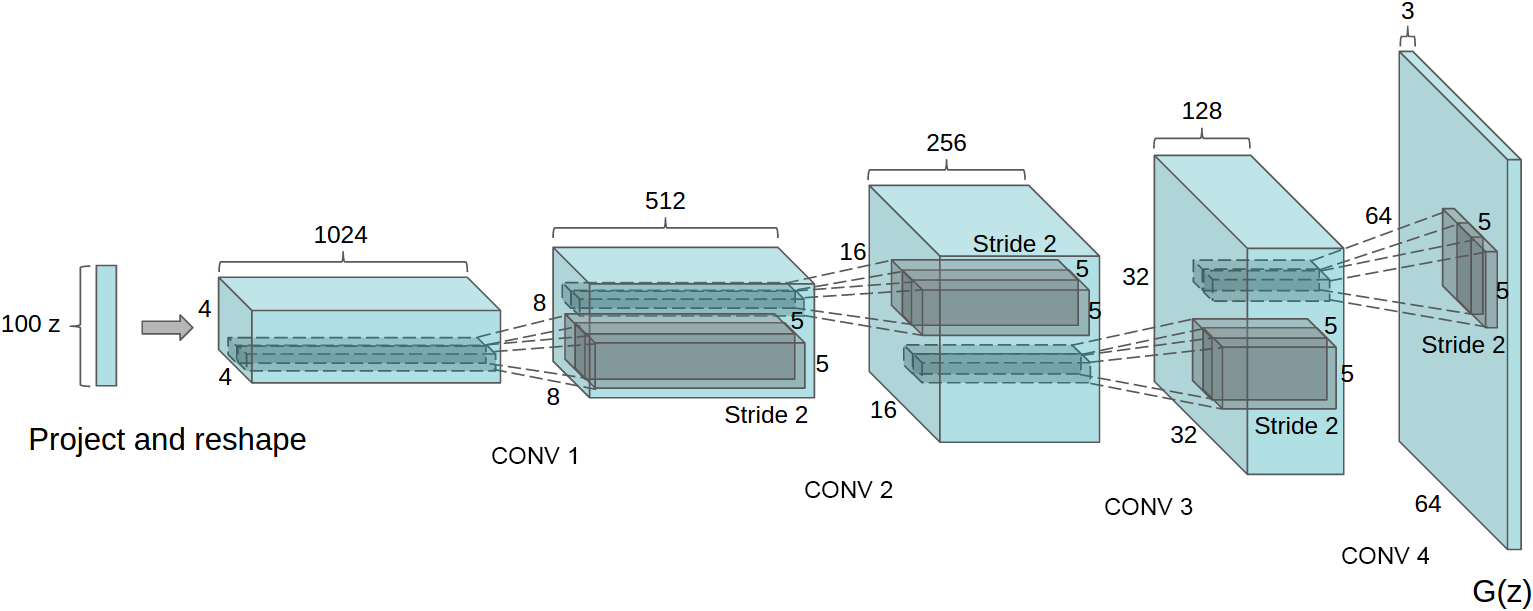
\includegraphics[width=0.8\textwidth]{figures/lsun_bedrooms_generator.png}
        \caption*{DCGAN architecture (Radford et al., 2015/2016).}
    \end{figure}
\end{frame}

% --- SLIDE 24.5.1 ---
\begin{frame}[t]{DCGAN}{Sample quality: MNIST \& faces}
    \only<1>{
        \begin{figure}
            \centering
            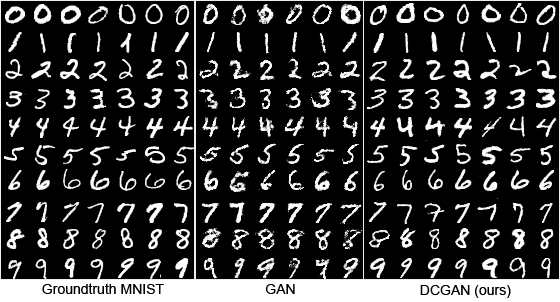
\includegraphics[width=0.9\linewidth]{figures/mnist_collage.png}
            \caption*{MNIST samples from DCGAN}
        \end{figure}
    }
    \only<2->{
        \begin{figure}
            \centering
            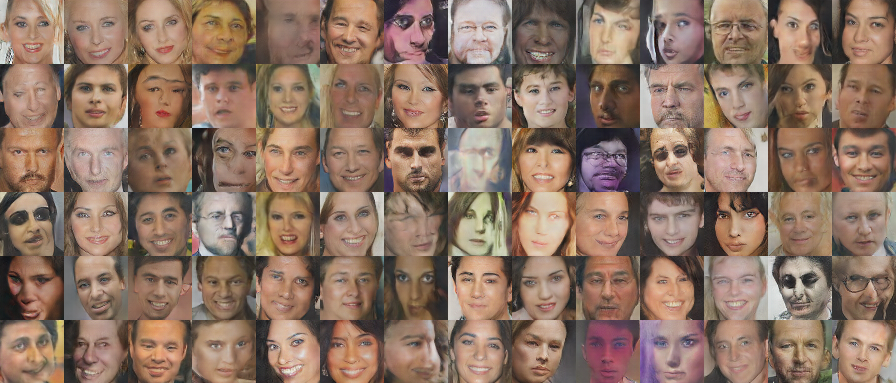
\includegraphics[width=0.6\linewidth]{figures/faces_128_filter_samples.png}
            \caption*{Faces (CelebA) from DCGAN}
        \end{figure}
        \only<3>{\textbf{Note:} quality improves markedly compared to early MLP GANs, but remains imperfect and at relatively low resolutions / latentdimensionalities. First decent generation in size 128x128}    }

\end{frame}

% --- SLIDE 25 ---
\begin{frame}{Progressive Growing of GANs}{Fade-in layers for high-resolution synthesis}
    \textbf{Key idea of \citet{karras_progressive_2018}:} progressively grow both the generator and discriminator during training.
    \begin{itemize}
        \item Train from low to high resolution (e.g., $4\times4\to8\times8\to\cdots\to1024\times1024$).
        \item \emph{Fade-in}: smoothly blend a newly added block over a transition period.
        \item Stabilizes training and improves high‑res detail; reduces compute at start.
        \item Generator: upsampling + conv blocks; Discriminator: mirror downsampling blocks.
    \end{itemize}
    \begin{figure}
        \centering
        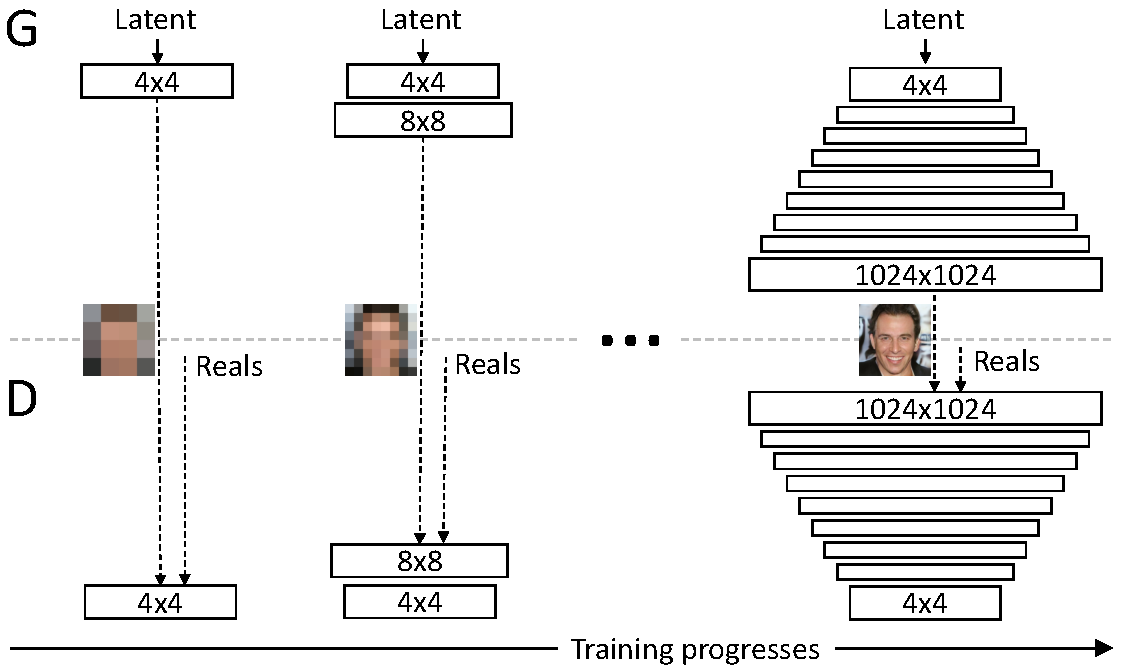
\includegraphics[width=0.5\linewidth]{figures/incremental.pdf}
        \caption*{Progressive growing architecture}
    \end{figure}
\end{frame}

% --- SLIDE 25.1 ---
\begin{frame}{Conditional Progressive Models}{Multi-scale super-resolution cascade}
    \begin{itemize}
        \item Conditional variants can be built as cascades of super‑resolution modules (e.g., $4\!\to\!8\!\to\!16\!\to\!\cdots$).
        \item Each stage upsamples and refines details conditioned on class/attributes.
        \item Useful for class‑conditional synthesis and guided upscaling.
    \end{itemize}
    \begin{figure}
        \centering
        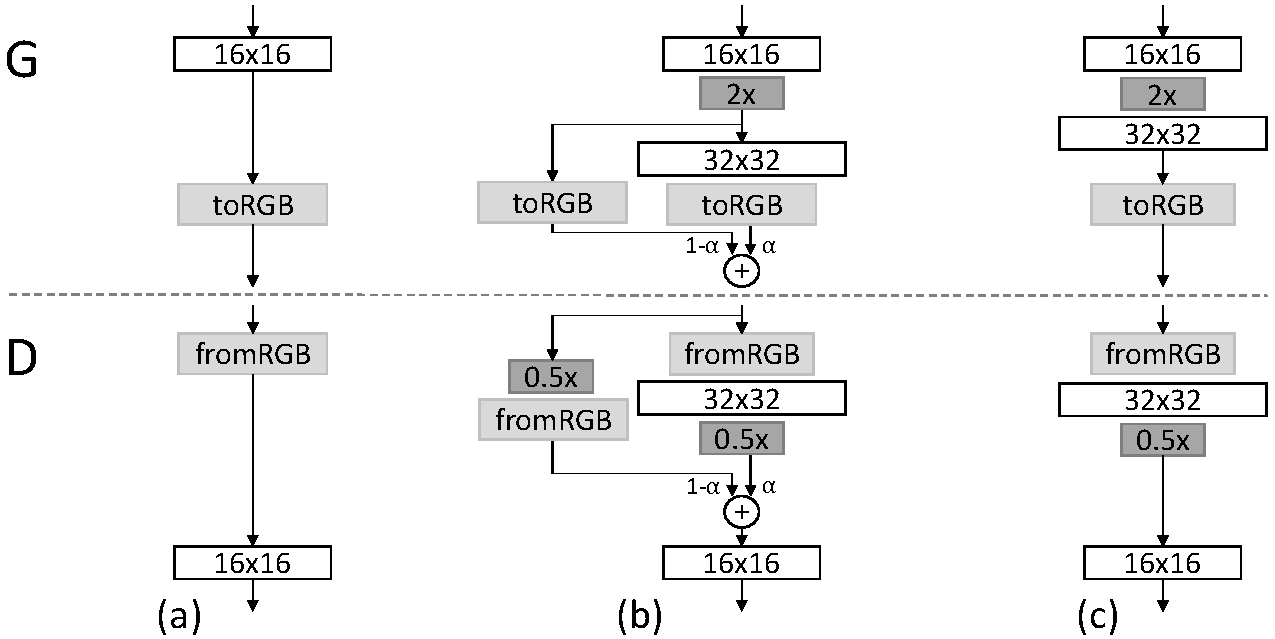
\includegraphics[width=0.6\linewidth]{figures/fadein.pdf}
        \caption*{Architectures of conditional super‑resolution models}
    \end{figure}
\end{frame}

% --- SLIDE 25.2 ---
\begin{frame}{Progressive Growing: Training Cost}{Time vs image size}
    \begin{figure}
        \centering
        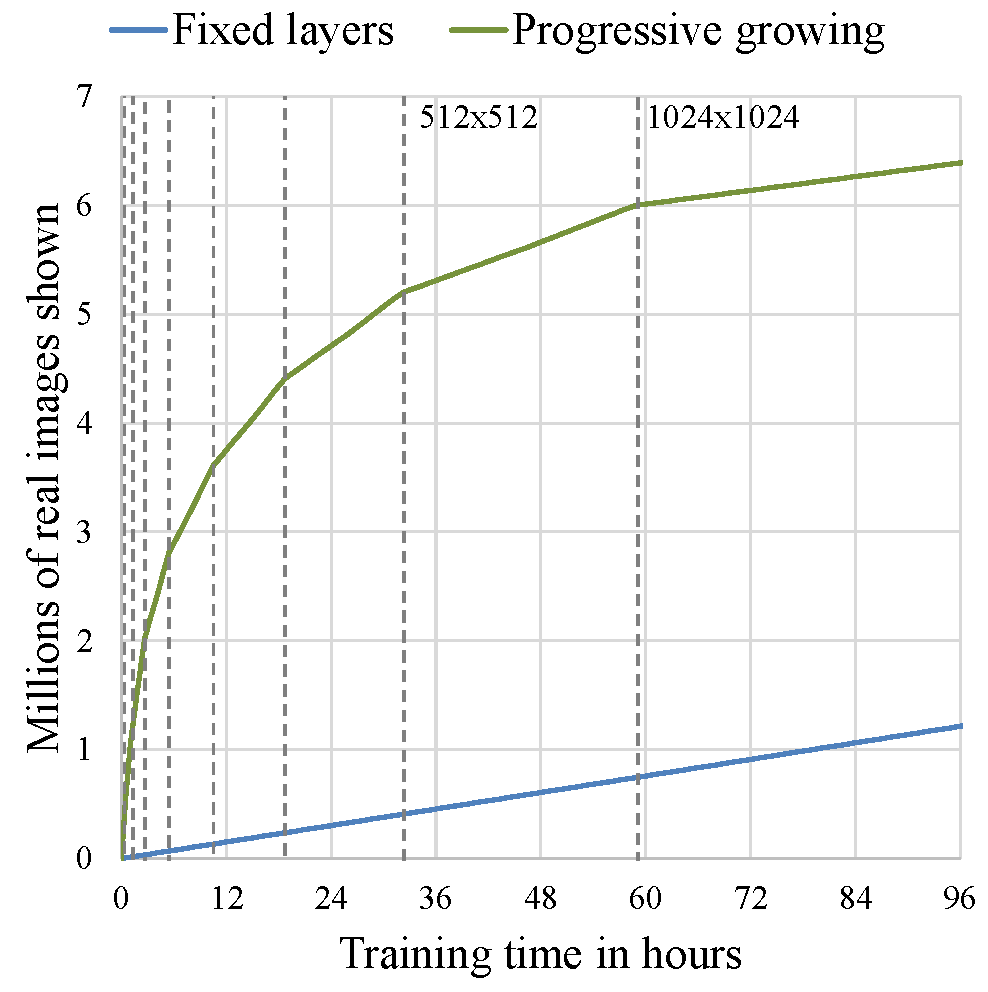
\includegraphics[width=0.5\linewidth]{figures/plot-perf-fixed-vs-grow2.pdf}
        \caption*{Training time as a function of image size}
    \end{figure}
    \textbf{Note:} early phases are cheap (small grids), heavy compute spent only at high resolutions.
\end{frame}

% --- SLIDE 25.3 ---
\begin{frame}{PGGAN Samples}{CelebA, LSUN}
    \only<1>{
        \textbf{Note:} PGGAN produces high-quality, high-resolution samples (1024x1024) with good global structure and fine details.
        \begin{figure}
            \centering
            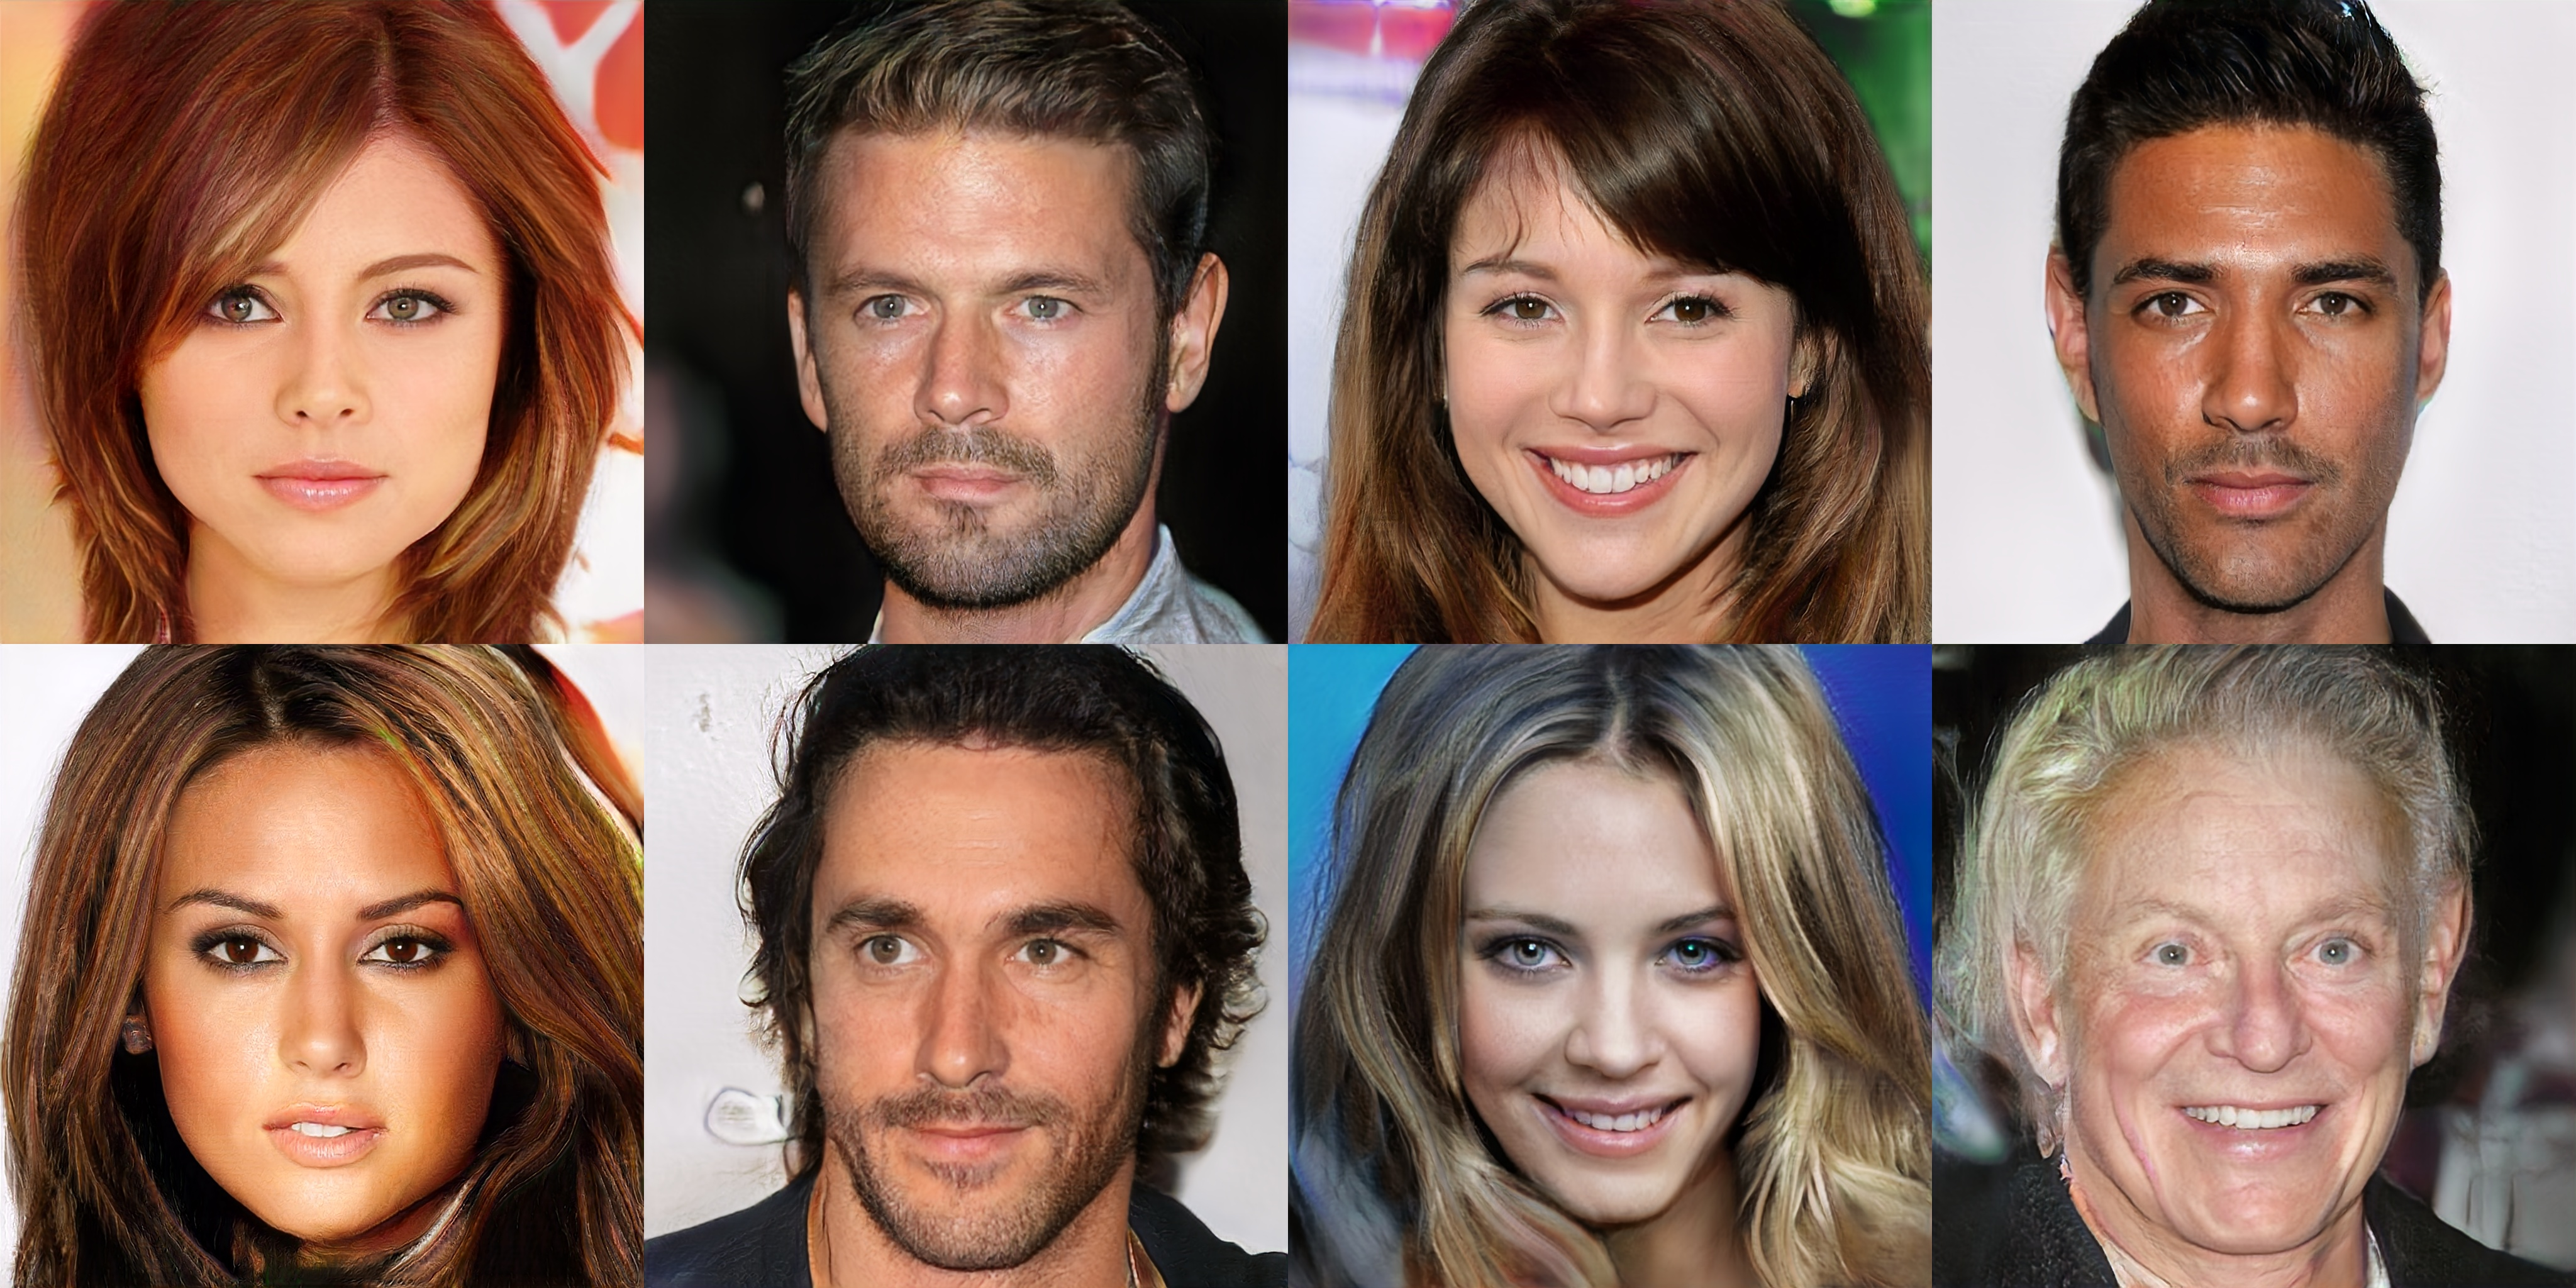
\includegraphics[width=0.95\linewidth]{figures/celeb1024-results.jpg}
            \caption*{CelebA}
        \end{figure}
    }
    \only<2-6>{
        LSUN dataset contains large-scale scene categories (bedrooms, churches, etc.) with diverse layouts and objects.
        \begin{figure}
            \centering
            \only<2>{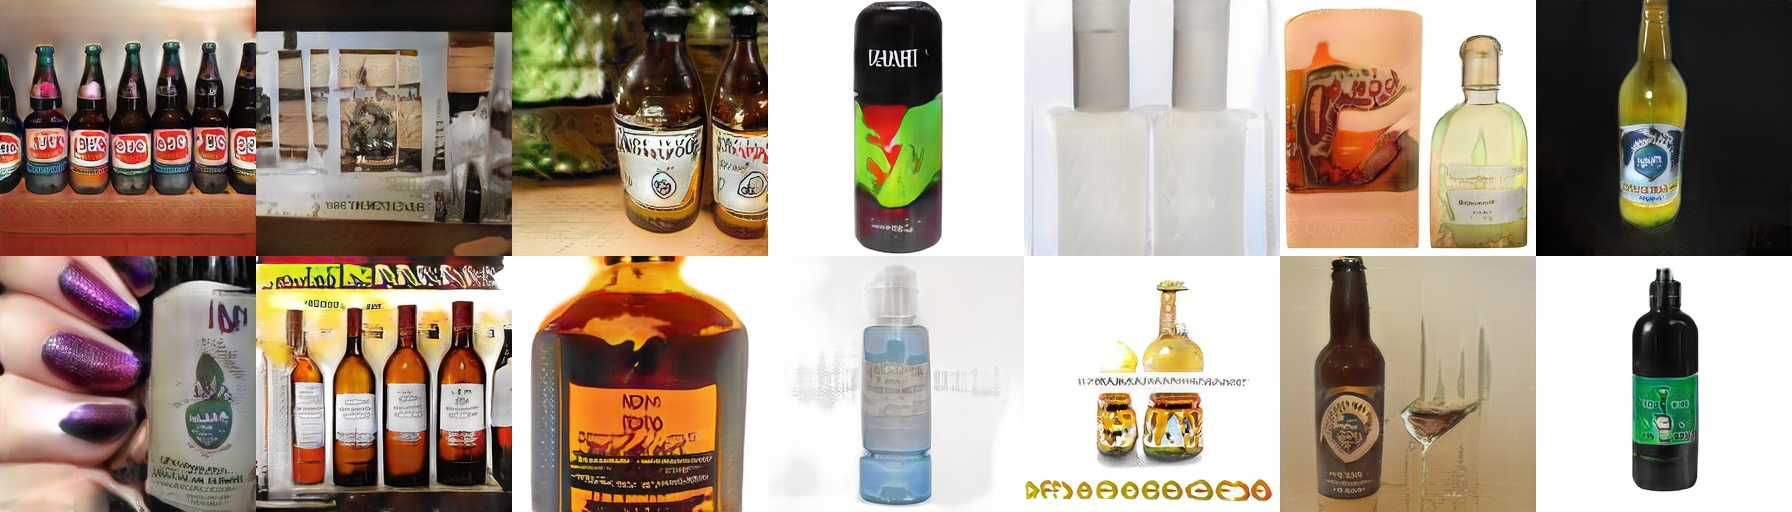
\includegraphics[width=0.95\linewidth]{figures/LSUNbottle.jpg}}
            \only<3>{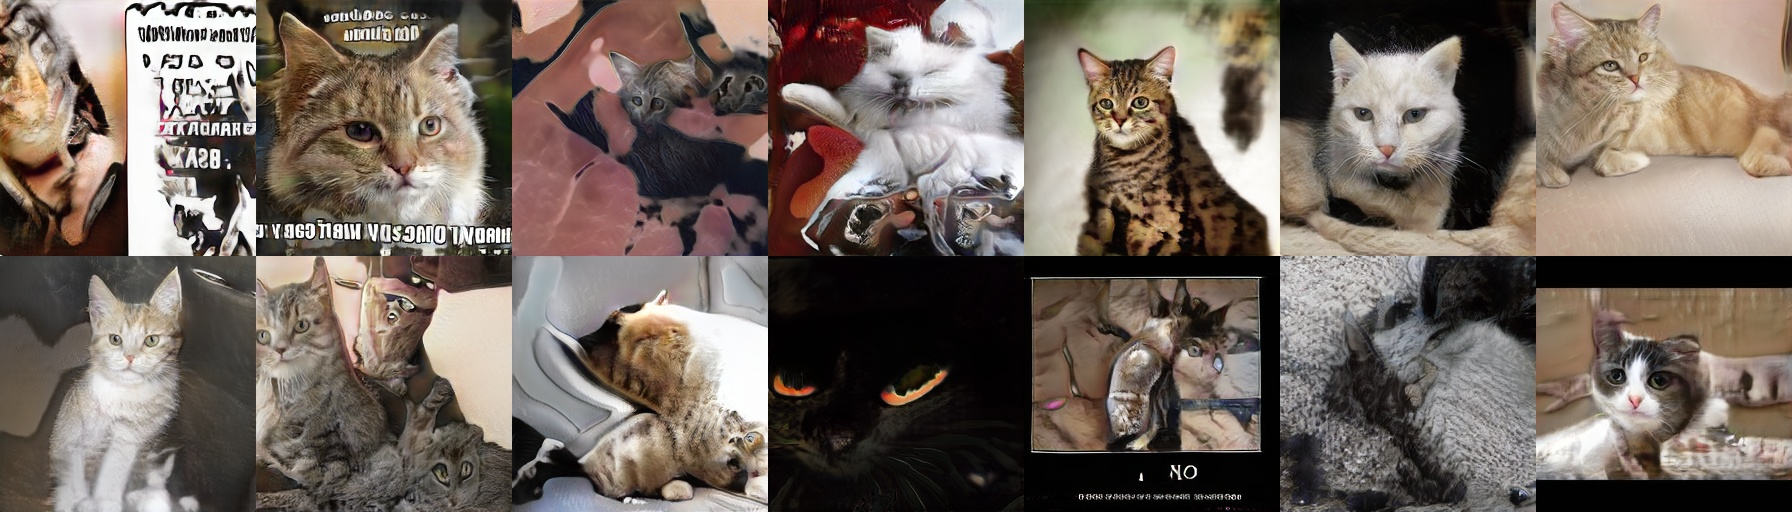
\includegraphics[width=0.95\linewidth]{figures/LSUNcat.jpg}}
            \only<4>{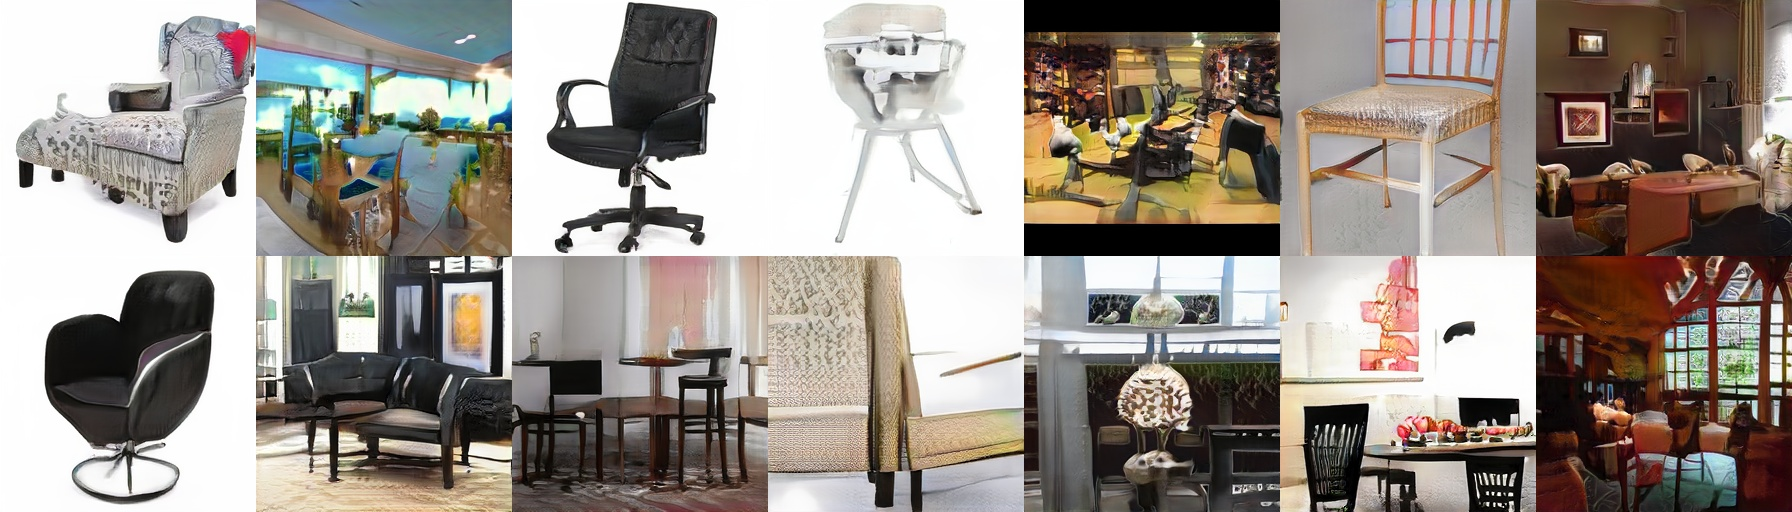
\includegraphics[width=0.95\linewidth]{figures/LSUNchair.jpg}}
            \only<5>{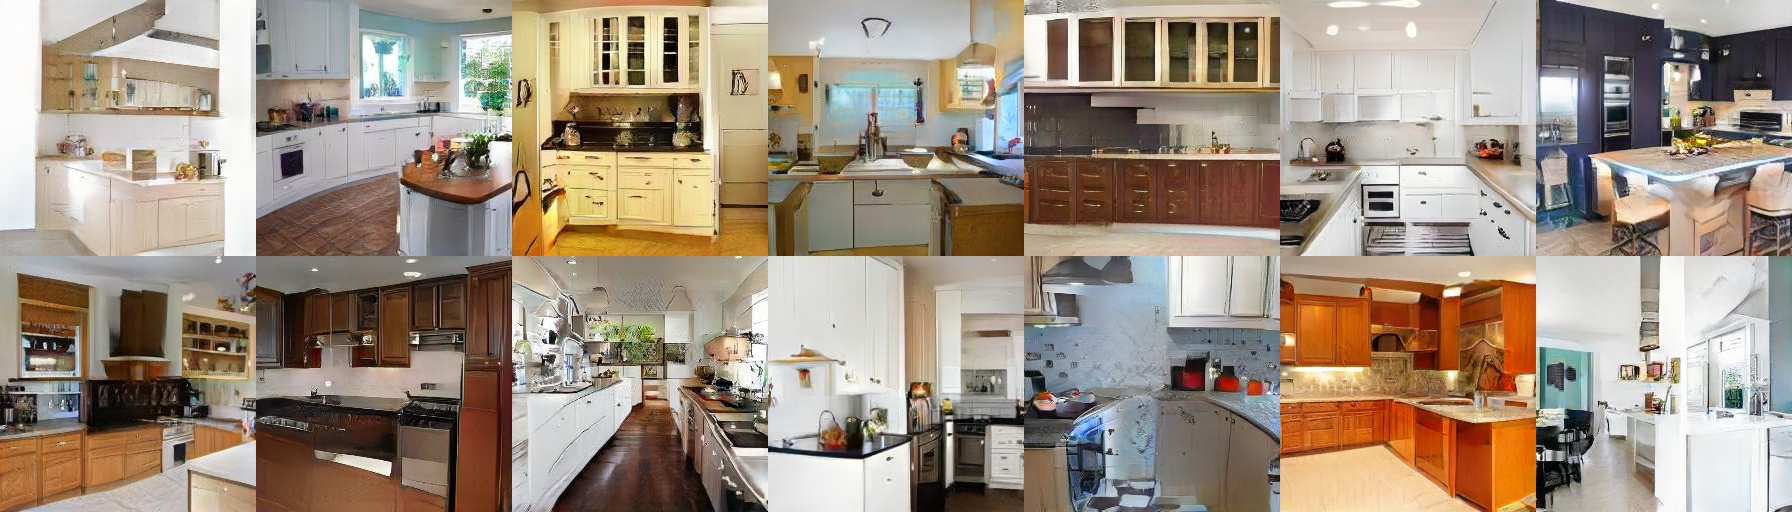
\includegraphics[width=0.95\linewidth]{figures/LSUNkitchen.jpg}}
            \only<6>{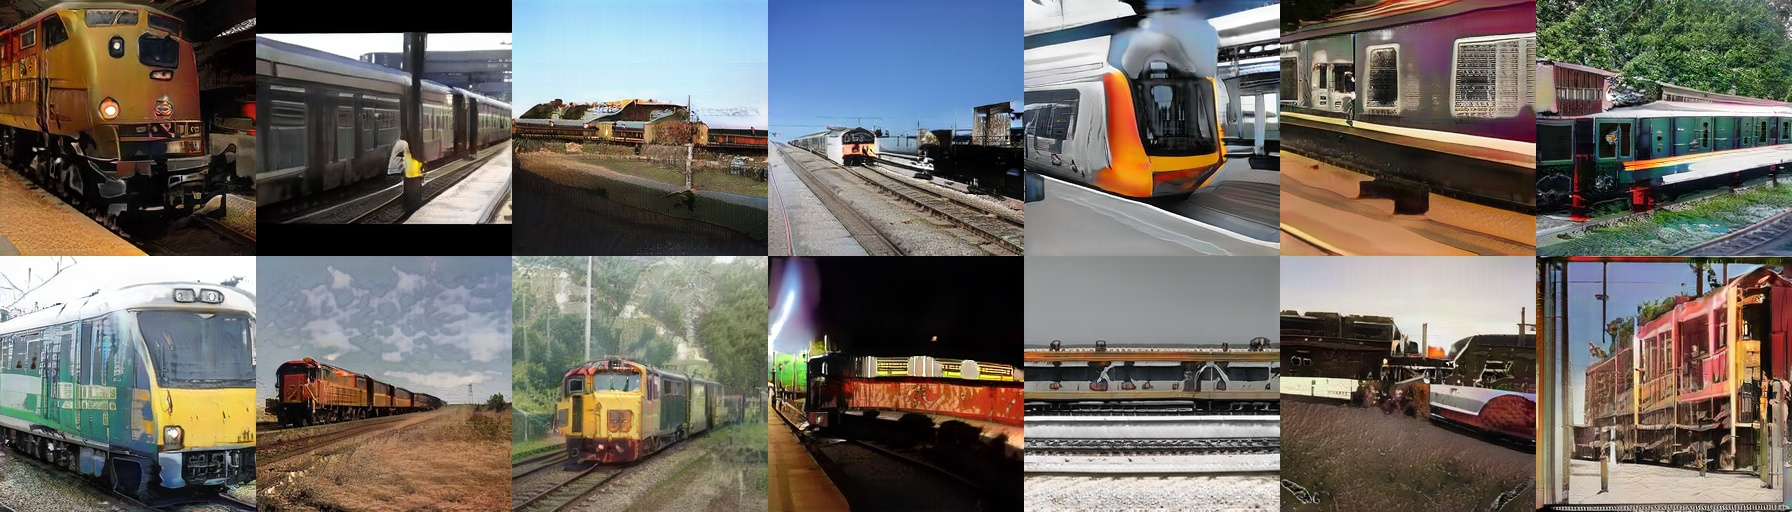
\includegraphics[width=0.95\linewidth]{figures/LSUNtrain.jpg}}
            \caption*{LSUN}
        \end{figure}
    }
\end{frame}

\vspace{0.5em}
% --- SLIDE 26 ---
\begin{frame}{BigGAN}{Class-conditional, attention, spectral norm}
    \textbf{Key improvements \citet{brock_large_2019}:}
    \begin{itemize}
        \item \textbf{Class-conditional architecture:} shared class embeddings + \emph{conditional BatchNorm} in $G$; deep residual blocks.
        \item \textbf{Long-range modeling:} non-local \emph{self-attention} layers (SAGAN-style) to capture global structure.
        \item \textbf{Stability \& fidelity:} \emph{spectral normalization} in $D$ \emph{and} $G$, very large-batch training, and the \emph{truncation trick} (trade-off between FID and diversity).
    \end{itemize}
    \begin{figure}
        \centering
        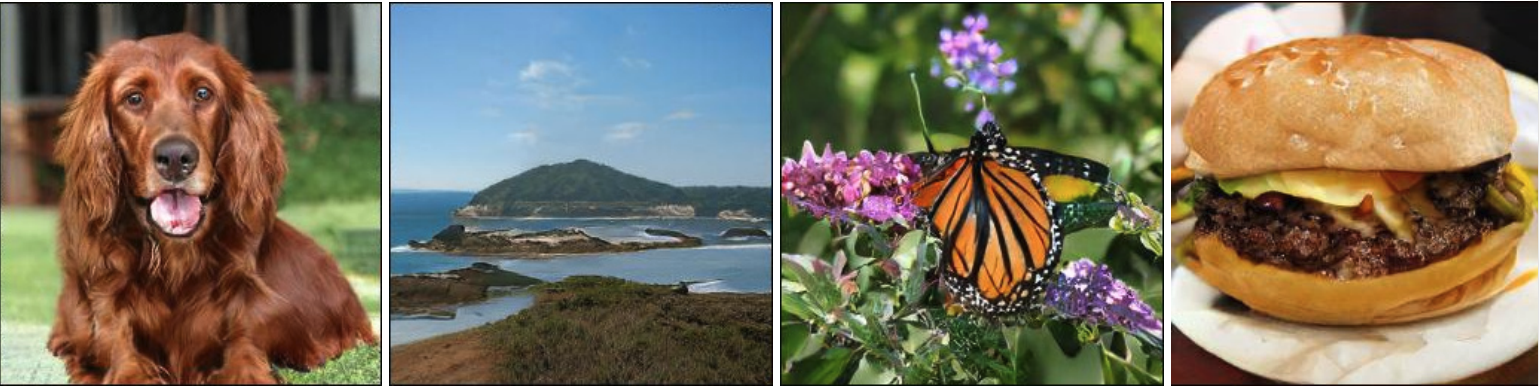
\includegraphics[width=0.7\linewidth]{figures/biggan.png}
        \caption*{BigGAN: class-conditional + attention + SN}
    \end{figure}
\end{frame}

% --- SLIDE 27 ---
\begin{frame}{StyleGAN \& StyleGAN-XL}{Style modulation, noise, path length reg}
    \textbf{Three milestones}
    \begin{itemize}
        \item \textbf{StyleGAN (2019):} style-based generator with mapping network; \emph{style modulation} (AdaIN) per layer; per-pixel noise for stochastic detail; improved disentanglement. \;(\citet{karras_style-based_2019})
        \item \textbf{StyleGAN2 (2020):} removes AdaIN artifacts via \emph{weight demodulation}; \emph{path length regularization}; architectural refinements for higher fidelity and fewer texture droplet artifacts. \;(\citet{karras_analyzing_2020})
        \item \textbf{StyleGAN-XL (2022):} scales StyleGAN to large, diverse datasets (e.g., ImageNet); stronger conditioning and training tricks; state-of-the-art FID/IS at higher resolutions. \;(\citet{sauer_stylegan-xl_2022})
    \end{itemize}
    \vskip 4pt
    Example of realism: \href{https://thispersondoesnotexist.com}{ThisPersonDoesNotExist.com} (StyleGAN faces).

\end{frame}

% --- SLIDE 28 ---
\begin{frame}{Domain Adaptation with GANs}{Motivation \& setup}
    \begin{itemize}
        \item \textbf{Goal:} translate from a \emph{source} domain $X$ to a \emph{target} domain $Y$ \emph{without} paired examples (unpaired domain adaptation).
        \item \textbf{Challenge:} many valid mappings $X\to Y$; need additional structure to avoid degenerate solutions.
        \item \textbf{Key idea:} use \emph{consistency losses} (cycle/identity) to regularize adversarial training.
    \end{itemize}
    \vskip 6pt
    \begin{figure}
        \centering
        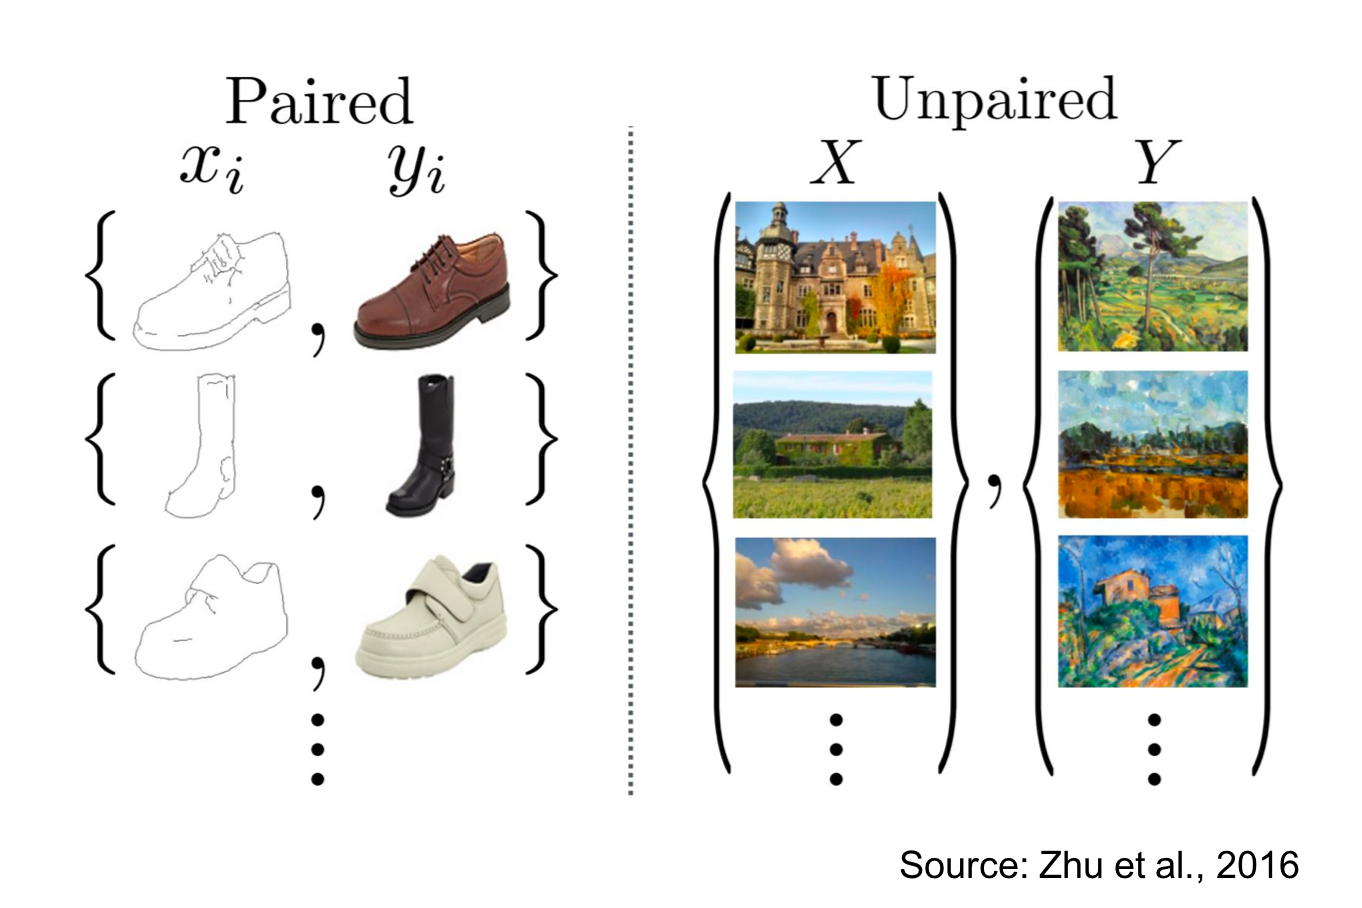
\includegraphics[width=0.6\linewidth]{figures/6.png}
        \caption*{Supervision regimes for domain adaptation}
    \end{figure}
\end{frame}

% --- SLIDE 29 ---
\begin{frame}{CycleGAN: Model}{Two generators, two discriminators}
    Let $G: X\to Y$ and $F: Y\to X$ with discriminators $D_Y$ and $D_X$.
    \begin{align*}
        \mathcal L_{\mathrm{GAN}}(G,D_Y) & = \E_{y\sim p_Y}[\log D_Y(y)] + \E_{x\sim p_X}[\log (1 - D_Y(G(x)))], \\
        \mathcal L_{\mathrm{GAN}}(F,D_X) & = \E_{x\sim p_X}[\log D_X(x)] + \E_{y\sim p_Y}[\log (1 - D_X(F(y)))].
    \end{align*}
    \vskip 4pt
    \begin{figure}
        \centering
        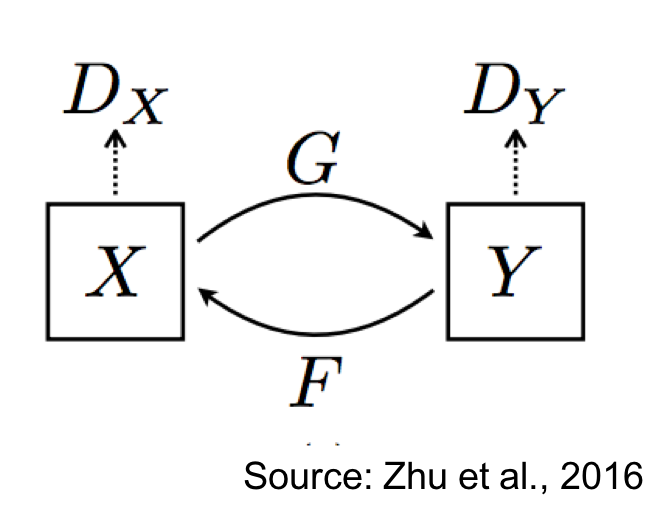
\includegraphics[width=0.5\linewidth]{figures/7.png}
        \caption*{Adversarial setup (two directions)}
    \end{figure}
\end{frame}

% --- SLIDE 30 ---
\begin{frame}{CycleGAN: Consistency Losses}{Why unpaired translation works}
    \textbf{Cycle-consistency:}
    \begin{equation*}
        \mathcal L_{\mathrm{cyc}}(G,F) = \E_{x\sim p_X}\big[\,\|F(G(x)) - x\|_1\,\big] + \E_{y\sim p_Y}\big[\,\|G(F(y)) - y\|_1\,\big].
    \end{equation*}

    \textbf{Total objective:}
    \begin{equation*}
        \min_{G,F}\max_{D_X,D_Y} \; \mathcal L_{\mathrm{GAN}}(G,D_Y)+\mathcal L_{\mathrm{GAN}}(F,D_X) + \lambda_\mathrm{cyc}\,\mathcal L_{\mathrm{cyc}} .
    \end{equation*}
    \vskip 4pt
    \begin{figure}
        \centering
        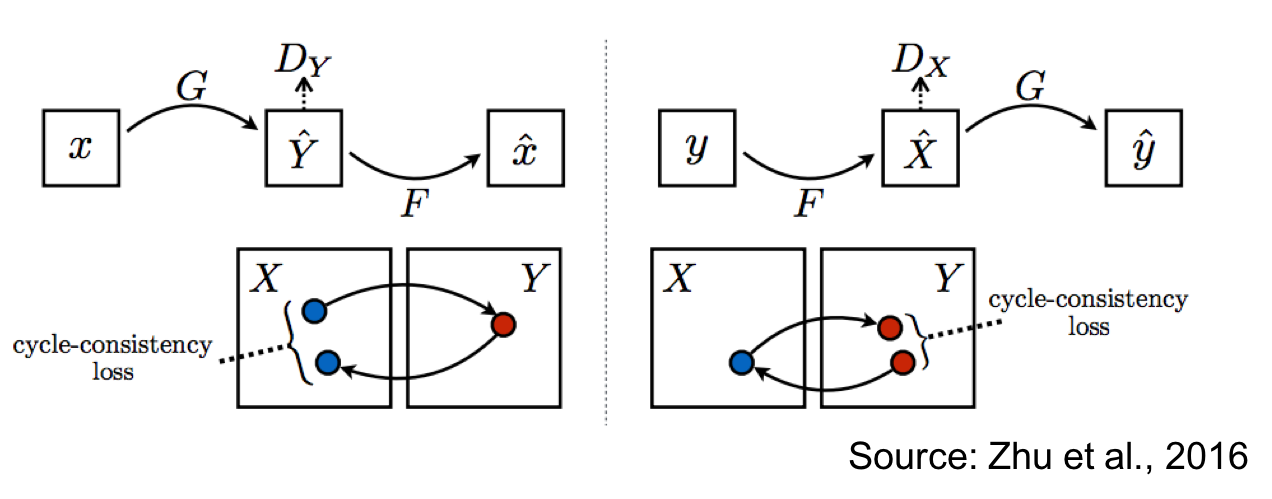
\includegraphics[width=0.75\linewidth]{figures/8.png}
        \caption*{Consistency regularization}
    \end{figure}
\end{frame}

% --- SLIDE 31 ---
\begin{frame}{CycleGAN: Qualitative Results}{Monet\,$\leftrightarrow$\,Photo; Horse\,$\leftrightarrow$\,Zebra; Summer\,$\leftrightarrow$\,Winter}
    \begin{figure}
        \centering
        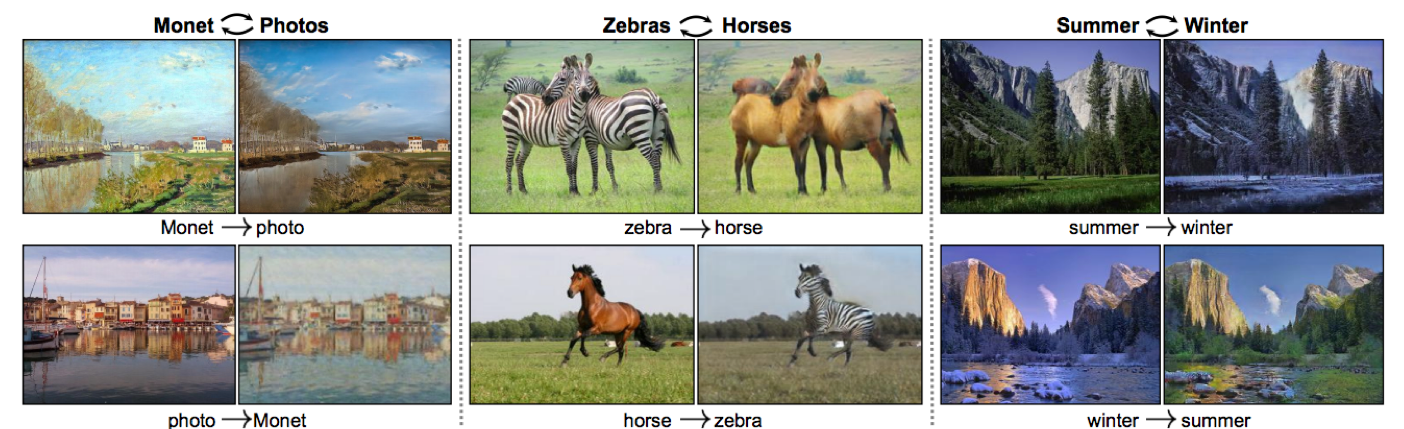
\includegraphics[width=0.8\linewidth]{figures/9.png}
        \caption*{Unpaired image-to-image translation}
    \end{figure}
\end{frame}

% --- SLIDE 31.5 ---
\begin{frame}{CycleGAN: Qualitative Results}{Photography\,$\leftrightarrow$\,Monet, Cezanne, Van Gogh, Ukiyo-e}
    \begin{figure}
        \centering
        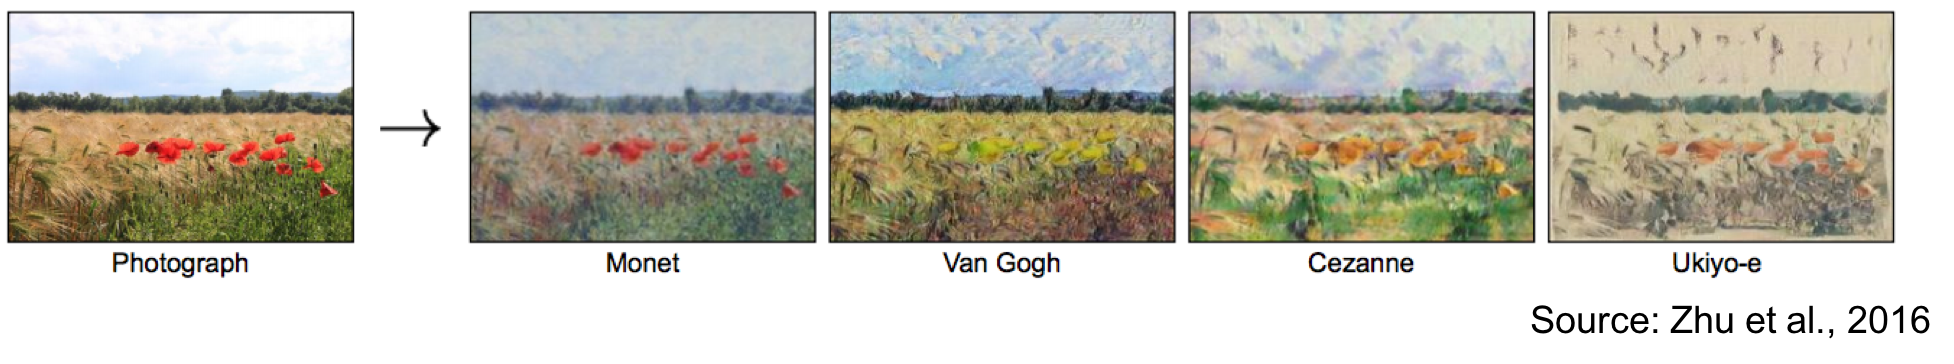
\includegraphics[width=0.8\linewidth]{figures/10.png}
        \caption*{Unpaired image-to-image translation}
    \end{figure}
\end{frame}

\begin{frame}{}{Your turn !}
    Get the Notebook on the course website and start working on it.
    \begin{itemize}
        \item \url{https://www.alexverine.com}
        \item Teaching
        \item Introduction to Deep Learning
        \item Lien Notebook
    \end{itemize}
    During this hands-on session we will train a GAN first on two dimensional data, and then on the MNIST dataset. Don't hesitate to use Colab or your own computer to run the notebook.
\end{frame}
